\chapter{Reading the Paper IV: Anatomy of a Spurious Floor}\label{ch:paper-spurious-floor}

\begin{chapterintro}
Suppose two lab groups time two quite different pendulums, one with a brass bob on a steel wire and one with a wooden bob on a string. One group reports a period of 2.321 s, the other 2.322 s. Two different systems agreeing to four digits is exciting: it suggests a hidden common cause, maybe a law. Then someone notices that both groups used the same stopwatch, and that the stopwatch had a fault that pushed every reading toward the same value. The "law" was a property of the instrument.

Section V of the paper \cite{soniR1} tells a story with exactly this shape. Two different non-Hermitian model classes, fitted to the Riemann zeros, stalled at in-sample error floors of 0.2321 and 0.2322 mean spacings. The near-identity invited a physical interpretation. The paper then takes the result apart, piece by piece: a dead parameter that fed on single-precision rounding noise, a plausible mechanism that fails by a factor of 2 to 7, an approximation used far outside its range of validity, and finally a fair refit that captures almost nothing. Nothing in this chapter is new mathematics. You already have every tool (second-order perturbation theory with an imaginary perturbation, the sum rule, PT symmetry and the null mode from Chapter~\ref{ch:non-hermitian}, floating-point precision from Chapter~\ref{ch:asymptotics}, least squares from Chapter~\ref{ch:least-squares}, Levenberg--Marquardt from Chapter~\ref{ch:fitting}). What is new is watching these tools used as a forensic kit.

Where this shows up in the paper: the method is in Sec.~II~E and Eq.~(5); the dissection is Sec.~V and its subsection V~A, with Fig.~5; the recipe is Appendix~A, steps 9--11, plus several "key anchors"; the abstract summarizes it in one sentence; and Sec.~VI records that this part was not rerun for the revision.
\end{chapterintro}

\begin{prerequisites}
\item Chapter~\ref{ch:non-hermitian}: the operator $H+iA$, imaginary first-order shifts, the second-order real shift, the quadratic form $-c^\top T^{(n)}c$, the sum rule $\sum_n\delta E_n=0$, PT symmetry, the null mode, exact diagonalization of complex matrices and matching by overlap.
\item Chapter~\ref{ch:perturbation}: Rayleigh--Schr\"odinger perturbation theory and its validity condition (matrix elements small compared with level spacings).
\item Chapter~\ref{ch:asymptotics}: machine epsilon ($2.2\times10^{-16}$ in double precision, $1.2\times10^{-7}$ in single precision, "float32") and how analytic zeros become rounding noise.
\item Chapters~\ref{ch:least-squares} and \ref{ch:fitting}: least squares as projection, the Jacobian, Levenberg--Marquardt damping, random restarts.
\item Chapters~\ref{ch:generalization} and \ref{ch:controls}: in-sample versus out-of-sample (OOS) error, the null model, exploratory versus confirmatory statements.
\item Chapters~\ref{ch:finite-differences}, \ref{ch:eigen} and \ref{ch:bound-states}: the finite-difference Hamiltonian, eigenvectors normalized by $\sum\psi^2h=1$, parity of states in an even potential, the infinite well.
\item Chapter~\ref{ch:probability}: rms, Pearson correlation, covariance.
\item Chapters~\ref{ch:paper-setup} and \ref{ch:paper-memorization}: the data, the target fluctuations, the in-sample null $0.2438$ on zeros 1--400.
\item First-year physics: decay laws, the idea of a damped oscillation.
\end{prerequisites}

%======================================================================
\section{What Section V is, and what it is not}\label{sec:paper-spurious-floor-scope}

Before reading any claim, read its scope. The paper is explicit. Section~V opens with:

\begin{quote}
``A subsidiary dissection reinforces the need for exact verification. This section is a methodological stress test of a second model class; the Hermitian conclusions of Secs.~III and~IV do not depend on it.''
\end{quote}

and the Discussion (Sec.~VI) adds that ``the non-Hermitian analysis of Sec.~V is inherited from the original computation and was not rerun for this revision.'' So three facts frame everything below.

\begin{enumerate}
\item The main results of the paper (fitted Hermitian potentials memorize, the explicit formula predicts) stand or fall independently of this section. If every number in Sec.~V were wrong, Tables~I--V would be untouched.
\item Section~V is about a \emph{method failure}, not about the zeros. Its lesson is how an optimization can produce an attractive but meaningless number, and how to catch it.
\item Its numbers come from the original submission's computation. The revision did not regenerate them. You should read them as carefully documented results of one pipeline, and note this when you weigh them (Chapter~\ref{ch:paper-critique} returns to this).
\end{enumerate}

\subsection{The story in five sentences}

(1) The paper fits a non-Hermitian correction $iA$ to the Wu--Sprung Hamiltonian, using the second-order formula Eq.~(5) for the real level shifts as a cheap stand-in (a \emph{surrogate}) for the exact spectrum. (2) Unconstrained fits on zeros 1--400 stall at in-sample rms floors 0.2321 (PT-odd class) and 0.2322 (absorptive-even class), against a null of 0.2438. (3) The second number turns out to be an artifact: a coefficient that should have no effect at all grew to $c_0\approx2.2\times10^6$ and harvested a small improvement from float32 rounding noise; after repair the even floor is 0.2358 and the coincidence disappears. (4) A natural mechanism for "why a floor at 0.232" fails quantitatively, and exact diagonalization of the fitted operators shows that the surrogate no longer describes them: their exact in-sample scores, 0.2523 and 0.2477, are worse than the null. (5) Fits redone inside amplitude limits where the surrogate is verified accurate capture only 1.9\% and 0.6\% over the null in exact spectra, so these model classes, treated fairly, are "empirically inert on this problem."

\Cref{tab:paper-spurious-floor-map} maps each claim to the section of this chapter that dissects it and to the earlier chapters that supply the tools.

\begin{table}[htbp]\centering
\caption{Claims of the paper's Sec.~V and where this chapter treats them.}\label{tab:paper-spurious-floor-map}
\small
\begin{tabular}{p{5.2cm}p{2.6cm}p{2.4cm}p{2.6cm}}
\toprule
Claim (paraphrased) & Paper location & This chapter & Tools from \\
\midrule
Second-order shift is a quadratic form in $c$ & Sec.~II E, Eq.~(5) & \cref{sec:paper-spurious-floor-surrogate} & Ch.~\ref{ch:perturbation}, \ref{ch:non-hermitian} \\
Unconstrained floors 0.2321, 0.2358; null 0.2438 & Sec.~V, para.~1 & \cref{sec:paper-spurious-floor-floors} & Ch.~\ref{ch:fitting}, \ref{ch:generalization} \\
Null-mode artifact, $c_0\approx2.2\times10^6$ & Sec.~V, para.~1; App.~A step 9 & \cref{sec:paper-spurious-floor-nullmode} & Ch.~\ref{ch:asymptotics}, \ref{ch:least-squares} \\
Sum rule, locality, block coherence fails & Sec.~V, V~A & \cref{sec:paper-spurious-floor-blocks} & Ch.~\ref{ch:non-hermitian}, \ref{ch:probability} \\
Surrogate invalid at fitted amplitude & Sec.~V; Fig.~5 left; step 11 & \cref{sec:paper-spurious-floor-exact} & Ch.~\ref{ch:eigen}, \ref{ch:non-hermitian} \\
Fair version is inert & Sec.~V; Fig.~5 right; step 10 & \cref{sec:paper-spurious-floor-fair} & Ch.~\ref{ch:linear-algebra}, \ref{ch:fitting} \\
Generic lessons & Sec.~V, last para. & \cref{sec:paper-spurious-floor-lessons} & Ch.~\ref{ch:controls} \\
\bottomrule
\end{tabular}
\end{table}

\subsection{Two words you need: "floor" and "null"}

Throughout Sec.~V the score is an \emph{in-sample} rms, measured on the training zeros 1--400, in units of the local mean spacing $\gap_n$ (recall from Chapter~\ref{ch:counting-zeros} that $\gap_n=ds_n/dn$, with $s_n$ the smooth zeros). The quantity to be explained is the target fluctuation
\begin{equation}
\mathrm{fluc}_n=\tilde t_n-E_n[\mathrm{smooth}],\label{eq:paper-spurious-floor-fluc}
\end{equation}
where $\tilde t_n$ is the bias-corrected target (Chapter~\ref{ch:finite-differences}) and $E_n[\mathrm{smooth}]$ is the $n$-th eigenvalue of the unperturbed Wu--Sprung Hamiltonian on the working grid (App.~A, step 12, uses exactly this definition). The \textbf{null} is the score of predicting no correction at all, that is, the rms of $\mathrm{fluc}_n/\gap_n$ over $n=1,\dots,400$. The paper's key anchors give it as $0.2438$.

A \textbf{floor} is the lowest in-sample rms an optimizer reaches before it stops improving, taken over restarts. A floor is a property of three things together: the model class, the data, and the optimizer. That sentence is the whole chapter in miniature.

\begin{pitfall}
Do not confuse this in-sample null (0.2438, zeros 1--400) with the out-of-sample null (0.2631 on zeros 401--500) used in Secs.~III and IV of the paper. Both are rms values of the same kind of fluctuation, but over different sets of zeros. Section~V's floors are all compared with 0.2438.
\end{pitfall}

\begin{keyideas}
\item Section~V is a subsidiary methodological stress test; the Hermitian conclusions do not depend on it, and it was not rerun in revision.
\item A floor is the in-sample rms at which an optimizer stalls; it reflects model, data and optimizer together.
\item All Sec.~V scores are in-sample on zeros 1--400 and are compared with the null 0.2438.
\end{keyideas}

%======================================================================
\section{The two non-Hermitian model classes}\label{sec:paper-spurious-floor-classes}

\subsection{What is being added to the Hamiltonian}

Recall the setting (Chapters~\ref{ch:schrodinger} and \ref{ch:wu-sprung}): in units $\hbar=2m=1$ the unperturbed Hamiltonian is $H=-d^2/dx^2+V(x)$, with $V$ the even Wu--Sprung potential on the box $[-L,L]$ with Dirichlet walls, $L=44.883$ at scale~1. Its eigenvalues $E_n$ are real and its normalized eigenfunctions $\psi_n(x)$ can be chosen real, because $H$ is a real symmetric operator (Chapter~\ref{ch:eigen}).

Sec.~II~E of the paper perturbs
\begin{equation}
H\;\to\;H+iA,\qquad A(x)=\sum_{k=0}^{M-1}c_k\,\phi_k(x),\label{eq:paper-spurious-floor-HiA}
\end{equation}
where $A(x)$ is a \emph{real} function of position, the $c_k$ are real coefficients to be fitted and the $\phi_k$ are basis functions. "Multiplication operator" means that $A$ acts on a wavefunction by multiplying it pointwise: $(A\psi)(x)=A(x)\psi(x)$. Because of the factor $i$, the operator $H+iA$ is not Hermitian, and its eigenvalues are in general complex (Chapter~\ref{ch:non-hermitian}).

The matrix elements of $A$ in the unperturbed basis are
\begin{equation}
A_{nm}=\langle n|A|m\rangle=\int_{-L}^{L}\psi_n(x)\,A(x)\,\psi_m(x)\,\dd x .\label{eq:paper-spurious-floor-Anm}
\end{equation}
Since $\psi_n$, $\psi_m$ and $A$ are all real, $A_{nm}$ is real, and swapping $n$ and $m$ does not change the integrand, so $A_{nm}=A_{mn}$. These two facts (real and symmetric) will be used again and again.

\begin{pitfall}
The paper uses the letter $A$ twice. In Sec.~II~C, $A_{nk}=\int|\psi_n|^2\phi_k\,\dd x$ is the first-order \emph{sensitivity matrix} of the Hermitian fit: rows are levels, columns are basis functions. In Sec.~II~E, $A$ is the \emph{operator} of \cref{eq:paper-spurious-floor-HiA}, and $A_{nm}$ is a matrix between two \emph{levels}. They are related (the diagonal $A_{nn}$ of the operator equals $\sum_k c_k\times$ the sensitivity entry $A_{nk}$), but they are different objects. Similarly $T^{(n)}$ below is a tensor, not the training window $T$ of Sec.~II~D and not a Chebyshev polynomial $T_k$.
\end{pitfall}

\subsection{The PT-odd class}

The first class uses
\begin{equation}
\phi_k(x)=\sin\!\Big(\frac{(k+1)\pi x}{L}\Big),\qquad k=0,1,\dots,M-1.\label{eq:paper-spurious-floor-odd}
\end{equation}
Every $\phi_k$ is an odd function: $\phi_k(-x)=-\phi_k(x)$. Notice the $k+1$. With $k$ instead, the $k=0$ function would be $\sin 0=0$, a basis function that is identically zero. The designers avoided that dead function here; keep this in mind, because the even class has a subtler dead function that was not avoided.

Recall from Chapter~\ref{ch:bound-states} that in an even potential every eigenfunction has definite parity, even or odd, alternating with $n$. Then $|\psi_n|^2$ is even, and for an odd $A$,
\begin{equation}
A_{nn}=\int_{-L}^{L}\underbrace{\psi_n(x)^2}_{\text{even}}\underbrace{A(x)}_{\text{odd}}\,\dd x=0,\label{eq:paper-spurious-floor-Ann0}
\end{equation}
because the integral of an odd function over a symmetric interval vanishes. This is the paper's "$A_{nn}=0$". More generally $A_{nm}\neq0$ only if $\psi_n\psi_m A$ is even, which for odd $A$ requires $\psi_n$ and $\psi_m$ of \emph{opposite} parity.

Why "PT"? Recall from Chapter~\ref{ch:non-hermitian}: parity P sends $x\to-x$ and time reversal T sends $i\to-i$ (complex conjugation). Applying P to $iA(x)$ gives $iA(-x)=-iA(x)$; applying T then gives $+iA(x)$. So $H+iA$ is unchanged by the combined operation PT when $A$ is odd. Its first-order shifts $iA_{nn}$ vanish, so its spectrum is real to leading order (the paper's words). We will see in \cref{sec:paper-spurious-floor-exact} that the spectrum stays exactly real for small enough amplitude and can turn complex beyond a threshold.

\subsection{The absorptive-even class}

The second class uses the even cosine basis familiar from the Hermitian fits,
\begin{equation}
\phi_k(x)=\cos\!\Big(\frac{k\pi x}{L}\Big),\qquad k=0,1,\dots,M-1,\label{eq:paper-spurious-floor-even}
\end{equation}
and the paper says it models $-i\Gamma/2$. Here is what that means. A complex potential $V(x)-i\Gamma(x)/2$ with $\Gamma(x)\ge0$ describes absorption: probability leaks out. To see this, use the time-dependent Schr\"odinger equation $i\,\partial\Psi/\partial\tau=\mathcal H\Psi$ (we write the time as $\tau$ to keep $t$ for the heights of zeros) with $\mathcal H=H-i\Gamma/2$:
\begin{align}
\frac{d}{d\tau}\int|\Psi|^2\dd x
&=\int\Big(\Psi^*\frac{\partial\Psi}{\partial\tau}+\Psi\frac{\partial\Psi^*}{\partial\tau}\Big)\dd x
\quad\text{(product rule)}\nonumber\\
&=\int\Big(\Psi^*(-iH\Psi-\tfrac{\Gamma}{2}\Psi)+\Psi(iH\Psi^*-\tfrac{\Gamma}{2}\Psi^*)\Big)\dd x
\quad\text{(insert }\partial_\tau\Psi=-i\mathcal H\Psi)\nonumber\\
&=-i\int\big(\Psi^*H\Psi-\Psi H\Psi^*\big)\dd x-\int\Gamma|\Psi|^2\dd x
\quad\text{(collect terms)}\nonumber\\
&=-\int\Gamma(x)|\Psi|^2\dd x\;\le\;0.
\quad\text{($H$ Hermitian, real: first integral is 0)}\label{eq:paper-spurious-floor-decay}
\end{align}
The first integral vanishes because $H$ is real and Hermitian, so $\int\Psi^*H\Psi\,\dd x=\int\Psi H\Psi^*\dd x$ (Chapter~\ref{ch:schrodinger}). Comparing $V-i\Gamma/2$ with $V+iA$ gives
\begin{equation}
A(x)=-\tfrac12\Gamma(x),\qquad\Gamma\ge0\iff A\le0\ \text{pointwise}.\label{eq:paper-spurious-floor-GammaA}
\end{equation}
That is the "physical constraint $\Gamma\ge0$ (i.e.\ $A\le0$ pointwise)" of Sec.~II~E.

For a single level, the eigenvalue $E_n-i\Gamma_n/2$ gives $\Psi\propto e^{-iE_n\tau}e^{-\Gamma_n\tau/2}$, so the \emph{width} $\Gamma_n=-2\,\Im(\text{eigenvalue})$ is the decay rate of $|\Psi|^2$. To first order the eigenvalue is $E_n+iA_{nn}$, so
\begin{equation}
\Gamma_n\approx-2A_{nn}=\int|\psi_n|^2\,\Gamma(x)\,\dd x .\label{eq:paper-spurious-floor-width}
\end{equation}
If $\Gamma(x)\ge0$ everywhere, every first-order width is non-negative. A negative width means growth, not decay: the "absorber" would be pumping probability in.

\begin{sample}{Parity kills the diagonal, and picks the partners}
Use the infinite well on $[-L,L]$ (RE3, Chapter~\ref{ch:bound-states}) with $L=\pi/2$, chosen so that the levels are $E_k=(k\pi/2L)^2=k^2$. The states are $\psi_k(x)=L^{-1/2}\sin\big(k\pi(x+L)/(2L)\big)$. Take one PT-odd mode, $A(x)=c\sin(\pi x/L)$. (a) Show that $A_{11}=A_{22}=0$. (b) Compute $A_{12}$. (c) Keeping only levels 1 and 2, estimate the second-order real shift of level 1 for $c=1$ using Eq.~(5) of the paper.

\textbf{Step 1: parity.} Substituting $u=(x+L)/(2L)\in[0,1]$, $\psi_k=L^{-1/2}\sin(k\pi u)$. Reflection $x\to-x$ is $u\to1-u$, and $\sin(k\pi(1-u))=\sin(k\pi)\cos(k\pi u)-\cos(k\pi)\sin(k\pi u)=-(-1)^k\sin(k\pi u)$. So $\psi_1$ is even and $\psi_2$ is odd. Since $\sin(\pi x/L)$ is odd, $\psi_1^2A$ and $\psi_2^2A$ are odd and integrate to zero: $A_{11}=A_{22}=0$.

\textbf{Step 2: rewrite the mode in $u$.} $\pi x/L=\pi(2u-1)=2\pi u-\pi$, so $\sin(\pi x/L)=-\sin(2\pi u)$. Also $\dd x=2L\,\dd u$.

\textbf{Step 3: the integral.}
\[
A_{12}=c\int_0^1\frac{\sin(\pi u)\sin(2\pi u)}{L}\big(-\sin 2\pi u\big)\,2L\,\dd u=-2c\int_0^1\sin(\pi u)\sin^2(2\pi u)\,\dd u .
\]
Use $\sin^2(2\pi u)=\tfrac12(1-\cos4\pi u)$ and $\sin a\cos b=\tfrac12[\sin(a+b)+\sin(a-b)]$:
\[
\int_0^1\sin(\pi u)\,\dd u=\frac{2}{\pi},\qquad
\int_0^1\sin(\pi u)\cos(4\pi u)\,\dd u=\tfrac12\Big[\frac{2}{5\pi}-\frac{2}{3\pi}\Big]=-\frac{2}{15\pi}.
\]
Hence $\int_0^1\sin(\pi u)\sin^2(2\pi u)\,\dd u=\tfrac12\big(\tfrac{2}{\pi}+\tfrac{2}{15\pi}\big)=\tfrac{16}{15\pi}$, and
\[
A_{12}=-\frac{32}{15\pi}\,c\approx-0.6791\,c .
\]

\textbf{Step 4: two-level second-order shift.} Eq.~(5) of the paper with one partner: $\delta E_1=-A_{12}^2/(E_1-E_2)=A_{12}^2/3$. For $c=1$:
\[
\boxed{\delta E_1\approx+0.1537,\qquad \delta E_2\approx-0.1537\ \text{(two-level estimate)}}
\]
Level 1 is pulled \emph{up} toward level 2 and level 2 pulled down: the opposite of Hermitian level repulsion. (Level 1 also couples to levels 4, 6, \dots, all of opposite parity; the two-level number is an estimate.)
\end{sample}

\begin{checkpoint}
In the PT-odd class, can level 1 and level 3 of an even potential couple through $A$?
\end{checkpoint}
\checkanswer{No. Levels 1 and 3 have the same parity (both even), so $\psi_1\psi_3$ is even and $\psi_1\psi_3A$ is odd for odd $A$; the integral vanishes. The odd class couples only opposite-parity pairs; the even class only same-parity pairs.}

\begin{keyideas}
\item The perturbation is $iA$ with $A(x)=\sum_kc_k\phi_k(x)$ real; its matrix $A_{nm}$ is real and symmetric.
\item PT-odd class: $\phi_k=\sin((k+1)\pi x/L)$, odd, so $A_{nn}=0$ and only opposite-parity levels couple.
\item Absorptive-even class: $\phi_k=\cos(k\pi x/L)$, modeling $-i\Gamma/2$; physics requires $\Gamma\ge0$, i.e.\ $A\le0$ pointwise, and first-order widths $\Gamma_n\approx-2A_{nn}$.
\end{keyideas}

%======================================================================
\section{The second-order surrogate and how it was fitted}\label{sec:paper-spurious-floor-surrogate}

\subsection{Re-deriving Eq.~(5)}

Chapter~\ref{ch:non-hermitian} derived Eq.~(5). Because everything in this chapter hinges on what that formula neglects, we re-derive it here in a form that works for any perturbation $W$, Hermitian or not.

Let $H_0$ have real eigenvalues $E_n$ (nondegenerate) and real orthonormal eigenvectors $|n\rangle$. Seek an eigenvalue $E$ of $H_0+W$ near $E_n$ with eigenvector written as $|\psi\rangle=|n\rangle+\sum_{m\ne n}a_m|m\rangle$ (we fix the coefficient of $|n\rangle$ to be 1; this is allowed because an eigenvector can be rescaled). Write $W_{km}=\langle k|W|m\rangle$.

\emph{Project onto $\langle n|$.} Using $\langle n|H_0=E_n\langle n|$ and $\langle n|m\rangle=\delta_{nm}$,
\begin{equation}
E_n+W_{nn}+\sum_{m\ne n}W_{nm}a_m=E .\label{eq:paper-spurious-floor-proj-n}
\end{equation}
\emph{Project onto $\langle k|$, $k\neq n$.}
\begin{equation}
E_ka_k+W_{kn}+\sum_{m\ne n}W_{km}a_m=Ea_k
\quad\Longrightarrow\quad
(E-E_k)\,a_k=W_{kn}+\sum_{m\ne n}W_{km}a_m .\label{eq:paper-spurious-floor-proj-k}
\end{equation}
\emph{Lowest order.} The $a_m$ are at least first order in $W$, so $\sum W_{km}a_m$ is second order; and $E-E_n$ is first order. Keeping only first-order terms,
\begin{equation}
a_k=\frac{W_{kn}}{E_n-E_k}+\order(W^2).\label{eq:paper-spurious-floor-ak}
\end{equation}
\emph{Insert into \cref{eq:paper-spurious-floor-proj-n}.}
\begin{equation}
E=E_n+W_{nn}+\sum_{m\ne n}\frac{W_{nm}W_{mn}}{E_n-E_m}+\order(W^3).\label{eq:paper-spurious-floor-RS2}
\end{equation}
Nothing here used $W^\dagger=W$; only the orthonormal basis of $H_0$ was used. Now set $W=iA$ with $A_{nm}$ real and symmetric:
\begin{align}
W_{nn}&=iA_{nn}\quad\text{(purely imaginary)},\label{eq:paper-spurious-floor-first}\\
W_{nm}W_{mn}&=(iA_{nm})(iA_{mn})=i^2A_{nm}^2=-A_{nm}^2\quad\text{(using }A_{mn}=A_{nm}).\label{eq:paper-spurious-floor-i2}
\end{align}
Therefore the real part of the eigenvalue, to second order, is $E_n+\delta E_n$ with
\begin{equation}
\boxed{\delta E_n=-\sum_{m\ne n}\frac{A_{nm}^2}{E_n-E_m}}\label{eq:paper-spurious-floor-eq5}
\end{equation}
which is Eq.~(5) of the paper (there written $|A_{nm}|^2$; for real $A_{nm}$ the two coincide). The sign is the reverse of Hermitian second-order theory: a partner above ($E_m>E_n$) pulls level $n$ \emph{up}, a partner below pulls it down. Levels attract.

\subsection{What the surrogate neglects: only even orders}

How large is the first neglected real term? Here is a short argument that it is fourth order, not third. Write $H(a)=H_0+iaA$, where $a$ scales the whole perturbation. In the unperturbed basis $H_0$ and $A$ are real matrices, so taking the complex conjugate of every entry gives
\begin{equation}
H(a)^*=H_0-iaA=H(-a).\label{eq:paper-spurious-floor-conj}
\end{equation}
If $H(a)v=Ev$, conjugating both sides gives $H(-a)v^*=E^*v^*$: the conjugate $E^*$ is an eigenvalue of $H(-a)$. Follow the eigenvalue $E_n(a)$ that starts at the real, nondegenerate $E_n$ when $a=0$. Its conjugate $E_n(a)^*$ also starts at $E_n$ and is an eigenvalue of $H(-a)$, so it is the branch $E_n(-a)$:
\begin{equation}
E_n(a)^*=E_n(-a)\quad\Longrightarrow\quad
\Re E_n(a)=\frac{E_n(a)+E_n(-a)}{2},\qquad
\Im E_n(a)=\frac{E_n(a)-E_n(-a)}{2i}.\label{eq:paper-spurious-floor-even-odd}
\end{equation}
The real part is an even function of $a$; the imaginary part is odd. A power series of an even function has only even powers. So
\begin{equation}
\Re E_n(a)=E_n+a^2\,\delta E_n^{(2)}+a^4\,\delta E_n^{(4)}+\dots,\label{eq:paper-spurious-floor-series}
\end{equation}
and the relative error of the surrogate is of order $a^2$ times (coupling/spacing)$^2$. Halving the amplitude cuts the relative error by about four; quartering it, by about sixteen. Remember this when you read "at quarter amplitude the surrogate is accurate."

\begin{beyond}
We used that a nondegenerate eigenvalue $E_n(a)$ of $H_0+iaA$ is a smooth (indeed analytic, i.e.\ given by a convergent power series) function of $a$ near $a=0$, so that "follow the branch" is meaningful and the series \cref{eq:paper-spurious-floor-series} exists. This is a theorem of analytic perturbation theory, due to Rellich and Kato; its proof needs complex analysis beyond this book. We take it on trust. The series converges only up to the nearest point (possibly complex) where two eigenvalues collide; \cref{sec:paper-spurious-floor-exact} shows such a collision explicitly.
\end{beyond}

For the PT-odd class there is more. Parity $P$ maps $x\to-x$; since $H_0$ is even and $A$ is odd, $PH(-a)P=H_0-iaA(-x)=H_0+iaA(x)=H(a)$. Similar matrices have the same eigenvalues, and parity maps the branch labelled $n$ to itself, so $E_n(-a)=E_n(a)$. Combined with \cref{eq:paper-spurious-floor-even-odd}, $E_n(a)^*=E_n(a)$: the eigenvalues of the PT-odd class are \emph{exactly real} for every amplitude below the first collision. Beyond it they may pair off into complex conjugates (PT symmetry breaking, Chapter~\ref{ch:non-hermitian}).

\subsection{The quadratic form and the tensors $T^{(n)}$}

Insert $A_{nm}=\sum_kc_k(\phi_k)_{nm}$, with $(\phi_k)_{nm}=\int\psi_n\phi_k\psi_m\,\dd x$, into \cref{eq:paper-spurious-floor-eq5}:
\begin{align}
A_{nm}^2&=\Big(\sum_kc_k(\phi_k)_{nm}\Big)\Big(\sum_lc_l(\phi_l)_{nm}\Big)=\sum_k\sum_lc_kc_l(\phi_k)_{nm}(\phi_l)_{nm},\nonumber\\
\delta E_n&=-\sum_k\sum_lc_k\,T^{(n)}_{kl}\,c_l=-c^\top T^{(n)}c,\qquad
T^{(n)}_{kl}=\sum_{m\ne n}\frac{(\phi_k)_{nm}(\phi_l)_{nm}}{E_n-E_m}.\label{eq:paper-spurious-floor-T}
\end{align}
Each level $n$ has its own $M\times M$ symmetric matrix $T^{(n)}$ (swapping $k$ and $l$ leaves the formula unchanged). The tensors depend only on the unperturbed potential, so they are computed once; after that, evaluating all 400 shifts for a trial $c$ costs only matrix--vector products, with no eigensolve. That is the attraction of a surrogate.

The paper adds a practical detail: the state sum $m$ runs ``over all 652 basis states with $E\le1000$ (truncating at 500 states measurably biases the top levels).'' The solvable example below shows why truncation biases the top.

\subsection{A solvable laboratory: one cosine in the box}

The infinite well gives exact matrix elements for the cosine modes. With $u=(x+L)/(2L)$ as in the sample problem above, $\cos(j\pi x/L)=\cos(2j\pi u-j\pi)=(-1)^j\cos(2j\pi u)$, and
\begin{align}
\langle k|\cos\tfrac{j\pi x}{L}|l\rangle
&=2(-1)^j\int_0^1\sin(k\pi u)\sin(l\pi u)\cos(2j\pi u)\,\dd u\nonumber\\
&=(-1)^j\int_0^1\big[\cos((k-l)\pi u)-\cos((k+l)\pi u)\big]\cos(2j\pi u)\,\dd u .\nonumber
\end{align}
For integers $a$ and $b\ge1$, $\int_0^1\cos(a\pi u)\cos(b\pi u)\,\dd u=\tfrac12$ if $|a|=b$ and $0$ otherwise (write the product as $\tfrac12[\cos((a-b)\pi u)+\cos((a+b)\pi u)]$ and integrate). Hence, for $j\ge1$,
\begin{equation}
\langle k|\cos\tfrac{j\pi x}{L}|l\rangle=\frac{(-1)^j}{2}\Big[\delta_{|k-l|,\,2j}-\delta_{k+l,\,2j}\Big].\label{eq:paper-spurious-floor-boxcos}
\end{equation}
So one cosine couples level $k$ to $k+2j$, to $k-2j$ when that is $\ge1$, and to $2j-k$ when that is $\ge1$ (with a minus sign); when $k=j$ the second term sits on the diagonal. Every coupling has magnitude $\tfrac12$.

Now take $A=c\cos(j\pi x/L)$ and levels $E_k=\kappa k^2$, $\kappa=(\pi/2L)^2$. For $n\neq j$ and $n\neq2j$, level $n$ has exactly two partners, $n+2j$ and $|n-2j|$, each with $A_{nm}^2=c^2/4$. The energy differences are
\[
E_n-E_{n+2j}=-4\kappa j(n+j),\qquad E_n-E_{|n-2j|}=\kappa\big(n^2-(n-2j)^2\big)=4\kappa j(n-j).
\]
Then \cref{eq:paper-spurious-floor-eq5} gives
\begin{align}
\delta E_n&=-\frac{c^2}{4}\Big[\frac{1}{-4\kappa j(n+j)}+\frac{1}{4\kappa j(n-j)}\Big]
=-\frac{c^2}{16\kappa j}\Big[\frac{1}{n-j}-\frac{1}{n+j}\Big]\nonumber\\
&=-\frac{c^2}{16\kappa j}\cdot\frac{2j}{n^2-j^2}
=-\frac{c^2}{8\kappa\,(n^2-j^2)} .\label{eq:paper-spurious-floor-onemode}
\end{align}
The two special levels are $n=j$ (only partner $3j$; also a first-order imaginary diagonal) and $n=2j$ (only partner $4j$, because $|2j-2j|=0$ is not a level). For them $\delta E_j=c^2/(32\kappa j^2)$ and $\delta E_{2j}=c^2/(48\kappa j^2)$.

\begin{sample}{The shift of level 5 from one cosine}
In the box with $L=\pi/2$ (so $\kappa=1$, $E_k=k^2$), take $A=\cos(\pi x/L)$, i.e.\ $j=1$, $c=1$. Find the second-order real shift of level 5 and check that perturbation theory is valid.

\textbf{Step 1: partners.} By \cref{eq:paper-spurious-floor-boxcos} with $j=1$, level 5 couples to levels 3 and 7, each with $A_{nm}=-\tfrac12$, so $A_{nm}^2=\tfrac14$.

\textbf{Step 2: sum.} $E_5-E_3=25-9=16$, $E_5-E_7=25-49=-24$:
\[
\delta E_5=-\tfrac14\Big[\frac{1}{16}+\frac{1}{-24}\Big]=-\tfrac14\cdot\frac{3-2}{48}=-\frac{1}{192}.
\]
This agrees with \cref{eq:paper-spurious-floor-onemode}: $-1/(8(25-1))=-1/192$.

\textbf{Step 3: validity.} The coupling $\tfrac12$ is small compared with the nearest spacing 16 (ratio $1/32$), so the fourth-order correction is of relative size about $(1/32)^2\approx10^{-3}$.
\[
\boxed{\delta E_5=-1/192\approx-0.00521}
\]
\end{sample}

\begin{sample}{The sum rule by hand, and the bias at the top}
Truncate the same problem ($j=1$, $c$ arbitrary, $E_k=k^2$) to the five states $k=1,\dots,5$. Compute all five second-order shifts in the truncated basis, check $\sum_n\delta E_n=0$, and compare levels 4 and 5 with their full-basis values.

\textbf{Step 1: pairs.} With $j=1$ the couplings are $(1,3)$, $(2,4)$, $(3,5)$ inside the truncated set (and $(4,6)$, $(5,7)$ lost), each with square $c^2/4$.

\textbf{Step 2: shifts.}
\begin{align*}
\delta E_1&=-\tfrac{c^2}{4}\cdot\tfrac{1}{1-9}=\tfrac{c^2}{32},&
\delta E_2&=-\tfrac{c^2}{4}\cdot\tfrac{1}{4-16}=\tfrac{c^2}{48},\\
\delta E_3&=-\tfrac{c^2}{4}\Big[\tfrac{1}{9-1}+\tfrac{1}{9-25}\Big]=-\tfrac{c^2}{64},&
\delta E_4&=-\tfrac{c^2}{4}\cdot\tfrac{1}{16-4}=-\tfrac{c^2}{48},\\
\delta E_5&=-\tfrac{c^2}{4}\cdot\tfrac{1}{25-9}=-\tfrac{c^2}{64}.
\end{align*}

\textbf{Step 3: sum.} $\tfrac{1}{32}+\tfrac{1}{48}-\tfrac{1}{64}-\tfrac{1}{48}-\tfrac{1}{64}=\tfrac{1}{32}-\tfrac{2}{64}=0$. The sum rule holds exactly.

\textbf{Step 4: full-basis values.} With all levels present, level 4 couples to 2 and 6 and level 5 to 3 and 7, so by \cref{eq:paper-spurious-floor-onemode} $\delta E_4=-c^2/120$ and $\delta E_5=-c^2/192$. The truncated values $-c^2/48$ and $-c^2/64$ are 2.5 and 3 times too negative: the missing upper partners would have pulled these levels up.
\[
\boxed{\text{truncated: }c^2\big(\tfrac1{32},\tfrac1{48},-\tfrac1{64},-\tfrac1{48},-\tfrac1{64}\big),\ \text{sum }0;\quad\text{top two biased low}}
\]
\end{sample}

\Cref{fig:paper-spurious-floor-truncation} shows the same effect with 30 states: the bulk agrees with the full basis, while the top two levels, which have lost their upper partners, are biased strongly downward (the top level by a factor larger than fifteen). This is the mechanism behind the paper's remark that truncating the state sum at 500 states ``measurably biases the top levels''; it is why the sum ran over 652 states.

\begin{figure}[htbp]\centering
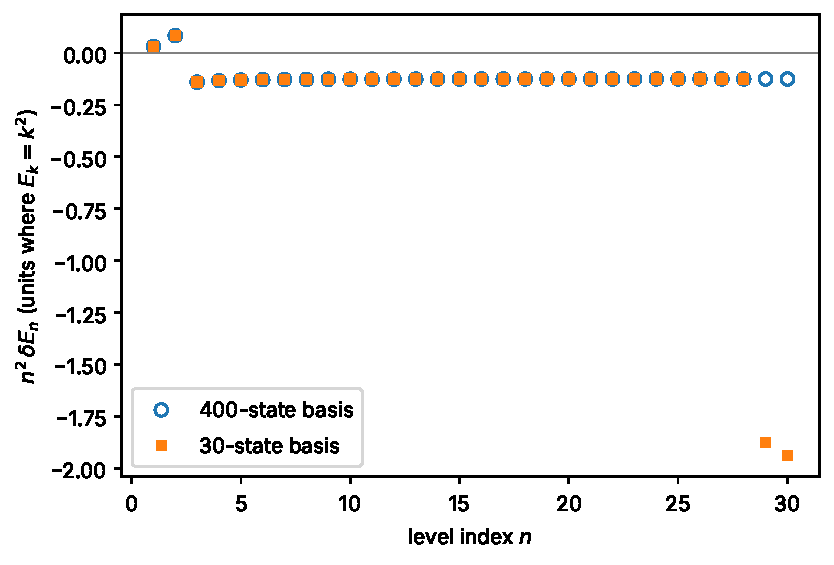
\includegraphics[width=0.85\linewidth]{figs/paper-spurious-floor_truncation.pdf}
\caption{Second-order real shifts $\delta E_n$ (multiplied by $n^2$ to make them visible) for a single cosine mode $A=\cos(\pi x/L)$ in the infinite well with $L=\pi/2$, computed in a 400-state basis (circles) and a 30-state basis (squares). Energies in units where $E_k=k^2$. The two curves agree except for the top two levels of the 30-state basis, which lack their upper coupling partners. Both sets of shifts satisfy $\sum_n\delta E_n=0$ over their own basis.}
\label{fig:paper-spurious-floor-truncation}
\end{figure}

\subsection{How the surrogate was fitted (Appendix A, step 10)}

The fit asks: which $c$ makes the surrogate shifts reproduce the target fluctuations? The residual of App.~A step 10 is
\begin{equation}
r_n(c)=\frac{\mathrm{fluc}_n+c^\top T^{(n)}c}{\gap_n},\qquad n=1,\dots,400 .\label{eq:paper-spurious-floor-rn}
\end{equation}
Read it as $(\mathrm{fluc}_n-\delta E_n)/\gap_n$ with $\delta E_n=-c^\top T^{(n)}c$: target minus model, in mean spacings. The Jacobian (Chapter~\ref{ch:fitting}) needs the derivative of the quadratic form. Writing it out with indices,
\begin{equation}
\frac{\partial}{\partial c_k}\sum_{i,l}c_iT_{il}c_l=\sum_lT_{kl}c_l+\sum_ic_iT_{ik}=2\,(T c)_k\quad\text{(using }T_{ik}=T_{ki}),\label{eq:paper-spurious-floor-grad}
\end{equation}
so $J_{nk}=\partial r_n/\partial c_k=2(T^{(n)}c)_k/\gap_n$, as the paper states. The update is Levenberg--Marquardt with "diag scaling" (Marquardt's form, Chapter~\ref{ch:fitting}): solve $(J^\top J+\lambda\,\mathrm{diag}(J^\top J))\,\delta c=-J^\top r$, trying damping values $(0.3\lambda,\lambda,10\lambda)$. Because the model is quadratic in $c$, the problem has many local minima, so the paper uses 6 random restarts with $c\sim\mathcal N(0,0.3^2)$ in each component, seed 0, at most 200 iterations.

\begin{sample}{One residual and its Jacobian}
Suppose for one level $\mathrm{fluc}_n=-0.6$, $\gap_n=1.5$, $M=2$, $T^{(n)}=\begin{pmatrix}2&1\\1&3\end{pmatrix}$ and $c=(1,-1)$. Find $r_n$ and the Jacobian row.

\textbf{Step 1: $T c$.} $T c=(2\cdot1+1\cdot(-1),\;1\cdot1+3\cdot(-1))=(1,-2)$.

\textbf{Step 2: quadratic form.} $c^\top Tc=1\cdot1+(-1)(-2)=3$, so the surrogate shift is $\delta E_n=-3$.

\textbf{Step 3: residual.} $r_n=(-0.6+3)/1.5=1.6$.

\textbf{Step 4: Jacobian.} $J_{n\cdot}=2(1,-2)/1.5=(1.333,-2.667)$. (A finite-difference check, $[r_n(c+he_k)-r_n(c-he_k)]/2h$, gives the same.)
\[
\boxed{r_n=1.6,\qquad J_{n\cdot}=(1.333,\,-2.667)}
\]
\end{sample}

\begin{pycode}
import numpy as np
# Box with L = pi/2, so E_k = k^2; one cosine mode j with coefficient c
K, j, c = 60, 1, 1.0
k = np.arange(1, K + 1)
E = k**2.0
kk, ll = np.meshgrid(k, k, indexing="ij")
A = c * (-1)**j / 2 * ((abs(kk - ll) == 2*j).astype(float)
                       - (kk + ll == 2*j).astype(float))
D = E[:, None] - E[None, :]
np.fill_diagonal(D, np.inf)          # exclude m = n
dE2 = -(A**2 / D).sum(axis=1)        # paper Eq. (5)
print("sum rule:", dE2.sum())        # zero to rounding
w, v = np.linalg.eig(np.diag(E) + 1j * A)
idx = np.argmax(abs(v), axis=1)      # exact state with largest weight on n
dE_exact = w[idx].real - E
print(dE2[:5])
print(dE_exact[:5])
\end{pycode}

\begin{keyideas}
\item Eq.~(5) follows from second-order perturbation theory with $W=iA$; $i^2=-1$ reverses the Hermitian sign, so coupled levels attract.
\item The real part of each eigenvalue is even in the amplitude, so the surrogate's first neglected term is fourth order and its relative error scales as amplitude squared.
\item PT-odd eigenvalues are exactly real until two levels collide.
\item $\delta E_n=-c^\top T^{(n)}c$ with symmetric tensors computed once; residual \cref{eq:paper-spurious-floor-rn}, Jacobian $2T^{(n)}c/\gap_n$.
\item Truncating the state sum biases the top levels; the paper summed over 652 states.
\end{keyideas}

%======================================================================
\section{The unconstrained floors}\label{sec:paper-spurious-floor-floors}

\subsection{What the paper reports}

Sec.~V, first paragraph:

\begin{quote}
``Unconstrained second-order non-Hermitian fits (Sec.~II~E) on zeros 1--400 stall at in-sample rms 0.2321 (PT-odd) and, after repairing the null-mode artifact, 0.2358 (absorptive-even), against a null of 0.2438; their OOS predictions are uncorrelated and can be wildly wrong (rms up to 1.4; up to 167 when fitting to 450 zeros, where extrapolated quadratic shifts blow up).''
\end{quote}

\textbf{In plain words.} The optimizer improved on doing nothing by only a small amount in-sample, and its predictions for zeros it did not see were useless, sometimes catastrophically so.

\textbf{Tools.} In-sample vs OOS and the null (Chapter~\ref{ch:generalization}); LM fitting (Chapter~\ref{ch:fitting}); the quadratic surrogate (\cref{sec:paper-spurious-floor-surrogate}).

\textbf{Computation behind it.} App.~A step 10, as described above, with the tensors of step 9.

\begin{sample}{How much did the floors capture?}
Using the paper's numbers, express each floor as a percentage improvement over the null 0.2438: (a) PT-odd 0.2321; (b) absorptive-even after repair 0.2358; (c) absorptive-even before repair 0.2322. (d) By what percentage did the artifact lower the even floor?

\textbf{Step 1: definition.} Capture $=(\text{null}-\text{floor})/\text{null}$.

\textbf{Step 2: compute.} (a) $(0.2438-0.2321)/0.2438=0.0117/0.2438=4.80\%$. (b) $0.0080/0.2438=3.28\%$. (c) $0.0116/0.2438=4.76\%$.

\textbf{Step 3: artifact.} $(0.2358-0.2322)/0.2358=0.0036/0.2358=1.53\%$.
\[
\boxed{4.80\%,\ 3.28\%,\ 4.76\%;\quad\text{artifact gain }1.53\%}
\]
These sit inside the paper's later statement that the floor is ``the null minus a small capture (3--7\% across splits).'' For contrast, the Hermitian fit with $M=400$ on the same zeros reaches in-sample 0.137 (Table~I of the paper), a capture of more than 40\%.
\end{sample}

\textbf{Why OOS can blow up.} In-sample, the data constrain the 400 numbers $c^\top T^{(n)}c$ for $n\le400$, not the vector $c$ itself. Directions of $c$ that barely affect these 400 quadratic forms can grow without penalty. A held-out level has its own tensor $T^{(n)}$, which can weight those directions strongly; since the shift is quadratic, a coefficient ten times too large gives a shift a hundred times too large. With 450 training zeros the paper reports held-out rms up to 167 mean spacings: far beyond any physical fluctuation, which is typically a fraction of a spacing. This is a heuristic explanation, consistent with the paper's phrase "extrapolated quadratic shifts blow up"; the paper does not give a detailed decomposition.

\begin{figure}[htbp]\centering
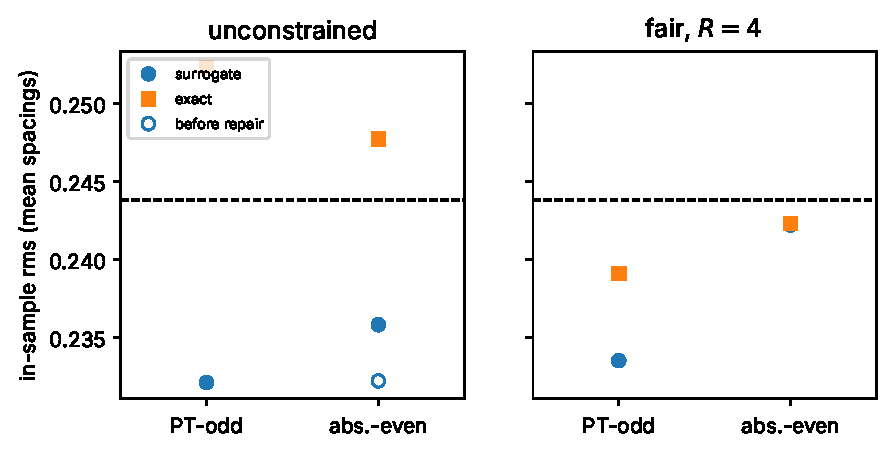
\includegraphics[width=0.85\linewidth]{figs/paper-spurious-floor_floors.pdf}
\caption{The paper's in-sample scores (rms in mean spacings, zeros 1--400) for the two non-Hermitian classes, redrawn from the numbers in Sec.~V and the key anchors of Appendix~A. "Surrogate" means scored with the second-order formula Eq.~(5); "exact" means scored with the exact eigenvalues of the fitted operator. The open marker is the even-class floor before the null-mode repair. Dashed line: null 0.2438. Lower is better.}
\label{fig:paper-spurious-floor-floors}
\end{figure}

\textbf{Strength and limits.} The floor values are reported to four digits and are anchored in App.~A, which makes them checkable against the Zenodo record \cite{zenodo}. The paper does not list $M$ for these fits in the main text, and the computation was not rerun in revision. The OOS figures (1.4, 167) are given as maxima ("up to"), not as a table.

\begin{keyideas}
\item Unconstrained floors: 0.2321 (odd), 0.2358 (even, repaired) against null 0.2438, captures of 4.8\% and 3.3\%.
\item OOS predictions are uncorrelated with truth and can explode because the shifts are quadratic in coefficients that the training data do not pin down.
\end{keyideas}

%======================================================================
\section{The null-mode artifact}\label{sec:paper-spurious-floor-nullmode}

\subsection{What the paper reports}

\begin{quote}
``Before repair, the absorptive-even floor sat at 0.2322, spuriously close to the PT-odd value: the optimizer had driven the exactly-null constant mode to $c_0\approx2.2\times10^6$, harvesting in-sample improvement from float32 noise in analytically-zero tensor entries. The apparent `identical floors across parity' dissolves.''
\end{quote}

\subsection{Why the constant mode should do nothing}

The even basis \cref{eq:paper-spurious-floor-even} starts with $\phi_0=\cos0=1$, the constant function. It is not identically zero (unlike $\sin0$), so it looks like a harmless basis function. But consider its effect.

\emph{Exactly}, with no perturbation theory: if $H\psi_n=E_n\psi_n$, then
\begin{equation}
(H+ic_0)\psi_n=E_n\psi_n+ic_0\psi_n=(E_n+ic_0)\psi_n .\label{eq:paper-spurious-floor-constshift}
\end{equation}
A constant imaginary potential shifts every eigenvalue by the same imaginary amount $ic_0$ and changes no eigenfunction. Its effect on every real part is zero to all orders.

\emph{In the surrogate}, the matrix of $\phi_0$ is
\begin{equation}
(\phi_0)_{nm}=\int\psi_n\cdot1\cdot\psi_m\,\dd x=\delta_{nm}\quad\text{(orthonormality)},\label{eq:paper-spurious-floor-phi0}
\end{equation}
so every off-diagonal element is zero and, from \cref{eq:paper-spurious-floor-T},
\begin{equation}
T^{(n)}_{0l}=\sum_{m\ne n}\frac{(\phi_0)_{nm}(\phi_l)_{nm}}{E_n-E_m}=\sum_{m\ne n}\frac{0\cdot(\phi_l)_{nm}}{E_n-E_m}=0\quad\text{for all }l,\label{eq:paper-spurious-floor-T0l}
\end{equation}
and by symmetry $T^{(n)}_{l0}=0$. The coefficient $c_0$ appears nowhere in $c^\top T^{(n)}c$. It is a \emph{dead parameter}: a null mode of the model.

\subsection{Why it was not dead in practice}

On a computer, $(\phi_0)_{nm}$ is computed as a sum $\sum_j\psi_n(x_j)\psi_m(x_j)h$ over grid points. In exact arithmetic, for exactly orthonormal eigenvectors, this is $\delta_{nm}$. In floating point it is $\delta_{nm}+\eta_{nm}$, where $\eta_{nm}$ is rounding noise. Recall from Chapter~\ref{ch:asymptotics} that the unit roundoff of single precision (float32) is about $1.2\times10^{-7}$, against $2.2\times10^{-16}$ in double precision. The paper's tensors were stored in float32 (Sec.~II~E: ``zeroed exactly rather than left as float32 noise''); the paper does not state why, and a common reason is memory, since float32 halves storage.

\Cref{fig:paper-spurious-floor-float32} shows the effect on a small example: the overlaps of 60 finite-difference eigenvectors of the infinite well, computed in float32 and in float64. The analytically-zero off-diagonal overlaps come out at the $10^{-8}$ level in float32 and many orders of magnitude smaller in float64.

\begin{figure}[htbp]\centering
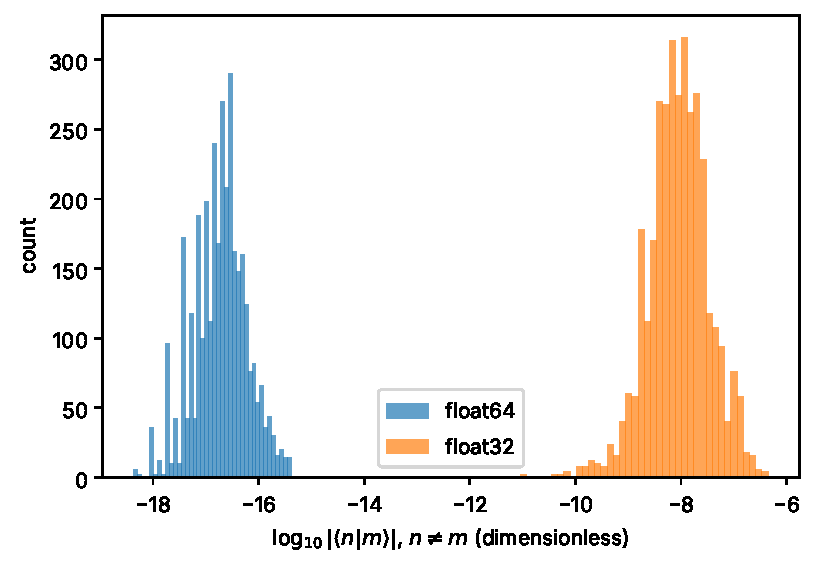
\includegraphics[width=0.85\linewidth]{figs/paper-spurious-floor_float32.pdf}
\caption{Histogram of $\log_{10}|\langle n|m\rangle|$ for $n\neq m$, the analytically zero overlaps of the first 60 finite-difference eigenvectors of the infinite well ($L=\pi/2$, $N=800$ interior points), each normalized so that $\sum\psi^2h=1$. Overlaps computed in float32 (right group) sit near $10^{-8}$; the same overlaps in float64 (left group) are near rounding level of double precision. A dead parameter multiplying such numbers is no longer dead.}
\label{fig:paper-spurious-floor-float32}
\end{figure}

\begin{pycode}
import numpy as np
from scipy.linalg import eigh_tridiagonal
L, N = np.pi/2, 800
h = 2*L/(N + 1)
d = 2/h**2 * np.ones(N)              # V = 0: infinite well
e = -1/h**2 * np.ones(N - 1)
E, psi = eigh_tridiagonal(d, e, select="i", select_range=(0, 59))
psi /= np.sqrt((psi**2).sum(axis=0) * h)   # sum psi^2 h = 1
G64 = psi.T @ psi * h
p32 = psi.astype(np.float32)
G32 = (p32.T @ p32) * np.float32(h)
off = ~np.eye(60, dtype=bool)
print("float64 median |offdiag|:", np.median(abs(G64[off])))
print("float32 median |offdiag|:", np.median(abs(G32[off])))
\end{pycode}

Once $(\phi_0)_{nm}=\eta_{nm}\ne0$ off the diagonal, the operator matrix becomes $A_{nm}=c_0\eta_{nm}+\sum_{l\ge1}c_l(\phi_l)_{nm}$. The constant mode now contributes a \emph{pseudo-random matrix} $c_0\eta_{nm}$. With entries $\eta\sim10^{-9}$ to $10^{-7}$, a coefficient $c_0=2.2\times10^6$ makes $c_0\eta$ of order $2.2\times10^{-3}$ to $0.26$ in energy units, comparable with level spacings of order 1. (This order-of-magnitude reading is ours; the paper states the mechanism, not this estimate.) A random matrix of the right size is a new, arbitrary set of features, and an unconstrained least-squares fit will use any feature that reduces the residual, however meaningless.

\subsection{Harvesting noise: a least-squares picture}

The essence can be seen in plain linear least squares (Chapter~\ref{ch:least-squares}).

\begin{sample}{Harvesting a noise column}
Fit $y=(0.3,-0.1,0.2,-0.4)$ with two columns: a genuine feature $g=(1,1,1,1)$ and a "noise" column $z_\varepsilon=\varepsilon\,(1,-1,-1,1)$ with $\varepsilon=10^{-7}$. Find the least-squares coefficients and the rms residual with and without the noise column.

\textbf{Step 1: orthogonality.} $g\cdot z_\varepsilon=\varepsilon(1-1-1+1)=0$, so the two coefficients decouple (projection onto orthogonal directions, Chapter~\ref{ch:least-squares}).

\textbf{Step 2: genuine coefficient.} $\beta_g=g\cdot y/g\cdot g=(0.3-0.1+0.2-0.4)/4=0$.

\textbf{Step 3: noise coefficient.} $z_\varepsilon\cdot y=\varepsilon(0.3+0.1-0.2-0.4)=-0.2\varepsilon$ and $z_\varepsilon\cdot z_\varepsilon=4\varepsilon^2$, so
\[
\beta_z=\frac{-0.2\varepsilon}{4\varepsilon^2}=-\frac{0.05}{\varepsilon}=-5\times10^{5}.
\]

\textbf{Step 4: residuals.} Without the noise column the residual is $y$ itself: rms $=\sqrt{(0.09+0.01+0.04+0.16)/4}=\sqrt{0.075}=0.2739$. The noise column removes $(z_\varepsilon\cdot y)^2/(z_\varepsilon\cdot z_\varepsilon)=0.04\varepsilon^2/4\varepsilon^2=0.01$ from the sum of squares, leaving $0.29$: rms $=\sqrt{0.0725}=0.2693$.
\[
\boxed{\beta_z=-5\times10^5,\quad \text{rms }0.2739\to0.2693}
\]
The improvement does not depend on $\varepsilon$ at all; only the coefficient does, as $1/\varepsilon$. Smaller noise means a larger coefficient, not a smaller harvest. That is exactly the signature in the paper: an absurdly large $c_0$ together with a small, real-looking in-sample gain.
\end{sample}

\Cref{fig:paper-spurious-floor-harvest} repeats this at the paper's scale of data: 400 random targets of rms about 0.24, fitted with 20 genuine smooth columns plus a growing number of noise columns of size $10^{-7}$. Every added noise column lowers the in-sample rms a little, and every noise coefficient is of order $10^5$.

\begin{figure}[htbp]\centering
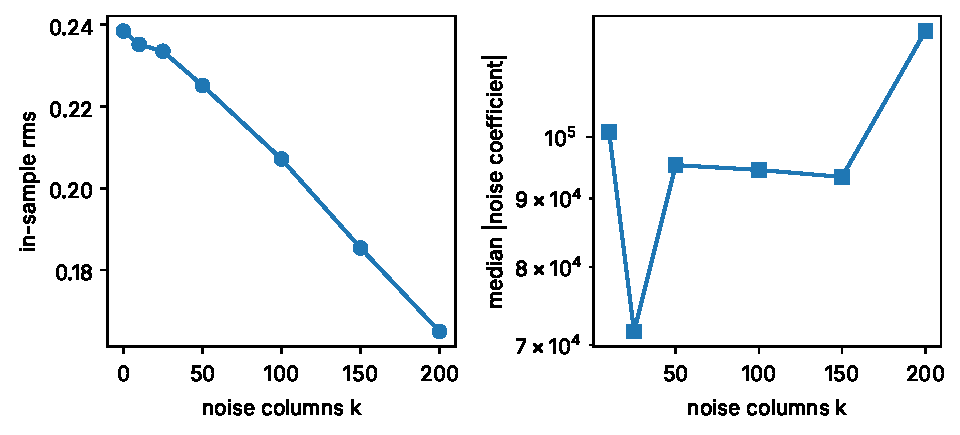
\includegraphics[width=0.95\linewidth]{figs/paper-spurious-floor_harvest.pdf}
\caption{Harvesting rounding-level noise by least squares. Left: in-sample rms of a fit to 400 random targets (rms about 0.24) with 20 smooth columns plus $k$ columns of Gaussian noise scaled by $10^{-7}$; the rms falls with every added column. Right: median magnitude of the fitted noise coefficients, of order $10^5$, i.e.\ inversely proportional to the noise scale. Data and noise drawn with \texttt{numpy.random.default\_rng(2)}.}
\label{fig:paper-spurious-floor-harvest}
\end{figure}

\subsection{The repair and what it revealed}

App.~A step 9: ``even-class rows $T^{(n)}_{0l}$ zeroed analytically.'' Setting those entries to their exact value, zero, makes $c_0$ truly dead again. After repair the even floor rose from 0.2322 to 0.2358, while the odd floor stayed at 0.2321 (the odd basis has no constant mode). The near coincidence 0.2321 versus 0.2322, which had suggested a parity-independent "floor" with physical meaning, was an artifact: it vanished when one input bug was fixed.

\begin{checkpoint}
Why does the constant mode have zero second-order real shift but a nonzero effect on the imaginary parts?
\end{checkpoint}
\checkanswer{Its matrix is the identity, $(\phi_0)_{nm}=\delta_{nm}$. The off-diagonal elements, which drive the second-order real shift, are zero; the diagonal elements, which give the first-order imaginary shift $ic_0$, are 1. Exactly, $H+ic_0$ has eigenvalues $E_n+ic_0$: all imaginary, no real change.}

\begin{checkpoint}
Two variants of a model report floors 0.2321 and 0.2322. List two checks you would make before attributing the agreement to physics.
\end{checkpoint}
\checkanswer{(i) Inspect the fitted coefficients for absurd magnitudes (a coefficient near $10^6$ on a mode that should be inert is a red flag). (ii) Recompute in higher precision, or zero analytically-null quantities, and see whether the numbers move. Also: score the exact operator rather than the surrogate.}

\textbf{Strength and limits.} The artifact claim is unusually strong for a diagnostic: the paper names the dead parameter, its value, the noise source, and the repair, and reports the score before and after. What the paper does not do is show that float32 noise alone produces exactly a 1.5\% gain; our least-squares illustration shows that such gains are generic, not that this one is quantitatively explained.

\begin{keyideas}
\item The constant mode $\phi_0=1$ is a null mode: exactly, $H+ic_0$ only shifts eigenvalues by $ic_0$; in the surrogate, $T^{(n)}_{0l}=0$.
\item In float32 the analytic zeros become noise near $10^{-8}$--$10^{-7}$; multiplied by $c_0\approx2.2\times10^6$ they act as a random operator of physical size.
\item Least squares harvests a fixed improvement from any noise column, with a coefficient scaling as $1/(\text{noise size})$.
\item After repair the even floor is 0.2358; the "identical floors across parity" dissolve.
\end{keyideas}

%======================================================================
\section{The block-coherence hypothesis and why it fails}\label{sec:paper-spurious-floor-blocks}

\subsection{The sum rule and locality (Sec.~V~A)}

Recall the sum rule from Chapter~\ref{ch:non-hermitian}. If $n$ and $m$ both run over the same truncated set $S$ of states,
\begin{align}
\sum_{n\in S}\delta E_n
&=-\sum_{n\in S}\sum_{\substack{m\in S\\m\ne n}}\frac{A_{nm}^2}{E_n-E_m}\nonumber\\
&=-\sum_{\substack{n,m\in S\\n<m}}A_{nm}^2\Big[\frac{1}{E_n-E_m}+\frac{1}{E_m-E_n}\Big]
\quad\text{(group each pair once; }A_{mn}^2=A_{nm}^2)\nonumber\\
&=0 .\label{eq:paper-spurious-floor-sumrule}
\end{align}
Each pair contributes equal and opposite amounts to its two members. The paper verifies this numerically at the fitted coefficients: $3.6\times10^{-15}$ (odd) and $1.4\times10^{-14}$ (even) in Sec.~V~A, summarized as "verified to $4\times10^{-15}$" in the main text. Numbers at this level are rounding of double-precision sums; they confirm both the identity and the code.

\emph{Locality}: with weights $w_{nm}=|A_{nm}|^2/|E_n-E_m|$, the paper finds that half the total weight lies within $|n-m|\le5$ (odd class) and $\le10$ (even), and 90\% within about 60 levels. So the surrogate mostly moves levels by trading shifts between near neighbors.

\subsection{The hypothesis}

Put the two facts together. If shifts sum to zero and are traded only locally, then the model output averaged over a block of $w$ consecutive levels should be close to zero. Such a model cannot produce a slowly varying, block-averaged pattern. So the part of the target that is block-averaged (the "block-coherent" part) should be unreachable, and perhaps the floor \emph{is} that part. This is the hypothesis Sec.~V tests: that the floor equals the rms of the locally averaged part of the target fluctuation.

To make it precise, write $d_n=\mathrm{fluc}_n/\gap_n$ and, for an odd window $w=2q+1$, define the centred moving average and its complement:
\begin{equation}
B_w(d)_n=\frac1w\sum_{i=-q}^{q}d_{n+i},\qquad F_w(d)_n=d_n-B_w(d)_n .\label{eq:paper-spurious-floor-BF}
\end{equation}
$B_w$ is the block-coherent part, $F_w$ the locally mean-free part.

\subsection{The block part is a lower bound, not a prediction}

Here is what the hypothesis can and cannot claim. Suppose an ideal local model produced outputs $m_n$ with $B_w(m)=0$ exactly. The residual $d-m$ then has $B_w(d-m)=B_w(d)-B_w(m)=B_w(d)$ (moving averages are linear). And a moving average cannot increase rms. Indeed, for each window, by the Cauchy--Schwarz inequality (Chapter~\ref{ch:probability}: the square of an average is at most the average of the squares),
\begin{equation}
\Big(\frac1w\sum_{i=-q}^{q}x_{n+i}\Big)^2\le\frac1w\sum_{i=-q}^{q}x_{n+i}^2 ,\label{eq:paper-spurious-floor-CS}
\end{equation}
and summing over all full windows, each $x_j^2$ appears in at most $w$ windows, each time with weight $1/w$, so $\sum_n B_w(x)_n^2\le\sum_jx_j^2$. Applied to $x=d-m$, the rms of the residual is at least the rms of $B_w(d)$, up to an edge factor $\sqrt{N/(N-w+1)}$ that is negligible for $N=400$. So the block-coherent rms is a \emph{lower bound} on what a perfectly local, sum-preserving model could achieve. The hypothesis was that the observed floor sits at this bound.

\subsection{The test}

Sec.~V~A decomposes the in-sample target fluctuation (rms 0.2438) by centred $w$-level moving averages and finds block-coherent rms
\[
0.108,\ 0.049,\ 0.033,\ 0.035,\ 0.019\qquad\text{for }w=3,5,7,9,13.
\]
All are far below 0.232. The main text summarizes: ``that component has rms only 0.03--0.11 spacings for averaging windows of 3--13 levels, never near 0.232,'' failing ``by a factor 2--7.'' The factor follows from $0.232/0.108=2.1$ and $0.232/0.033=7.0$. (A careful reader notices that the $w=13$ value 0.019 lies below the quoted range 0.03--0.11 and would give a factor of about 12; the qualitative conclusion only gets stronger.)

The lower bound is nowhere near binding. The floor is not explained by what the model cannot do; it must be explained by what the model, as fitted, does not do.

\Cref{fig:paper-spurious-floor-blocks} repeats the decomposition at small scale with qmnt, using $d_n=(t_n-s_n)/\gap_n$ for zeros 1--400. This is the smooth-zero version of the target, not the paper's Richardson-corrected one, so it is close to but not identical with the paper's $d_n$. Its block-coherent rms stays below 0.15 for every window, far below the floor.

\begin{figure}[htbp]\centering
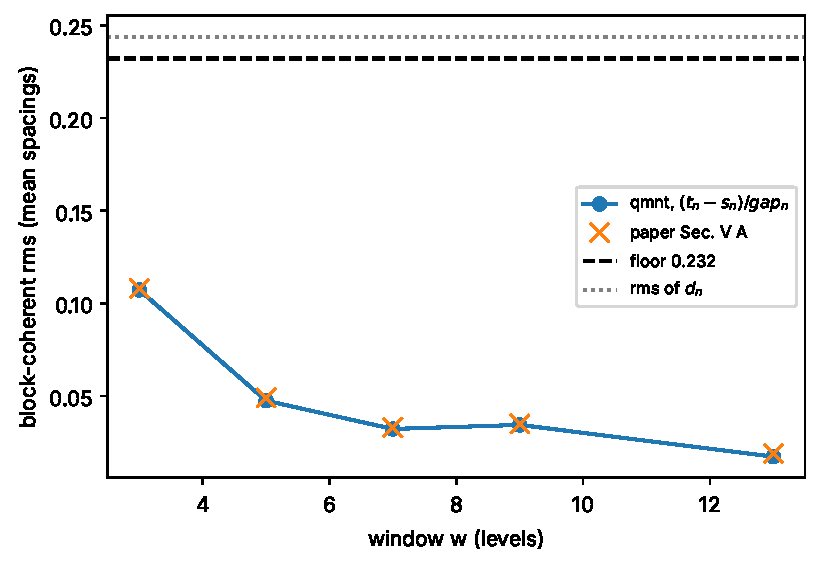
\includegraphics[width=0.85\linewidth]{figs/paper-spurious-floor_blocks.pdf}
\caption{Block-coherent rms (rms of the centred $w$-level moving average) of the zero fluctuations $d_n=(t_n-s_n)/\gap_n$, zeros 1--400, computed with qmnt (circles), and the values reported in the paper's Sec.~V~A for its corrected targets (crosses). Dashed: the unconstrained floor 0.232. Dotted: rms of $d_n$ itself. Moving averages use only full windows. The block-coherent part is several times smaller than the floor for every window.}
\label{fig:paper-spurious-floor-blocks}
\end{figure}

\begin{sample}{Why negatively correlated sequences have small block averages}
Let $d_n=(-1)^na$, the extreme of negative lag-1 correlation. Compute $B_w(d)$ and its rms for odd $w=2q+1$.

\textbf{Step 1: one window.} $B_w(d)_n=\frac aw\sum_{i=-q}^{q}(-1)^{n+i}=\frac{(-1)^na}{w}\sum_{i=-q}^{q}(-1)^i$.

\textbf{Step 2: the alternating sum.} The terms for $i$ and $-i$ are equal, so $\sum_{i=-q}^{q}(-1)^i=1+2\sum_{i=1}^{q}(-1)^i$. For $q$ odd the inner sum is $-1$, giving $-1$; for $q$ even it is $0$, giving $+1$. So the sum is $(-1)^q$.

\textbf{Step 3: rms.} $B_w(d)_n=(-1)^{n+q}a/w$, so $|B_w|=a/w$ for every $n$:
\[
\boxed{\mathrm{rms}\,B_w(d)=\frac{a}{w}}
\]
For $w=3$ the block part is one third of the signal. Recall from Chapter~\ref{ch:level-statistics} and the paper's Sec.~III that the zero fluctuations have negative autocorrelation at lags 1--3; that is why their block averages are small.
\end{sample}

\subsection{The $p=2$ oscillation is itself local}

The paper adds: ``The dominant $p=2$ oscillation, period $2\pi/\log2\approx9$ in $t$, is only $\sim$6--7 levels at these heights, itself a local pattern.'' Check it. The period in $t$ is $2\pi/\log2=9.065$ (RE2). The number of levels in one period is the period divided by the mean spacing $\gap_n=2\pi/\log(s_n/2\pi)$. With qmnt, $\gap_{200}\approx1.516$ and $\gap_{400}\approx1.341$, so one period spans about 6.0 levels near $n=200$ and about 6.8 levels near $n=400$. A pattern that repeats every six or seven levels averages out over windows of comparable size, so it contributes little to the block-coherent part; and it is a pattern a local redistribution could in principle produce. Locality is not what stops the model.

\subsection{Capture, not mechanism}

The paper's conclusion: ``The floor is simply the null minus a small capture (3--7\% across splits), not a physically meaningful constant.'' And from Sec.~V~A: ``The fitted models' output correlates $\approx+0.3$ with the locally mean-free component but with rms only 0.06--0.075: capture, not mechanism, limits the floor.'' The next sample shows that these numbers are self-consistent.

\begin{sample}{Is a weak capture enough to make the floor?}
Model the target as $d=B+F$ with $B$ and $F$ uncorrelated, $\mathrm{rms}(d)=0.2438$, $\mathrm{rms}(B)=0.033$ (the $w=7$ value). Let the model output $m$ have rms $\sigma_m$, correlation $\rho=0.3$ with $F$, and zero correlation with $B$. (These simplifying assumptions are ours, not the paper's.) Find the residual rms for $\sigma_m=0.07$ and $0.06$, and the $\sigma_m$ that minimizes it. Treat all sequences as mean-zero.

\textbf{Step 1: rms of $F$.} Uncorrelated parts add in square: $\sigma_F^2=0.2438^2-0.033^2=0.059438-0.001089=0.058349$, so $\sigma_F=0.2416$.

\textbf{Step 2: residual variance.} $\sigma_r^2=\mathrm{var}(d-m)=\sigma_d^2-2\,\mathrm{cov}(d,m)+\sigma_m^2$, and $\mathrm{cov}(d,m)=\mathrm{cov}(F,m)+\mathrm{cov}(B,m)=\rho\sigma_F\sigma_m+0$.

\textbf{Step 3: numbers.} For $\sigma_m=0.07$: $\sigma_r^2=0.059438-2(0.3)(0.2416)(0.07)+0.0049=0.054193$, $\sigma_r=0.2328$. For $\sigma_m=0.06$: $\sigma_r=0.2331$.

\textbf{Step 4: optimum.} $d\sigma_r^2/d\sigma_m=-2\rho\sigma_F+2\sigma_m=0$ gives $\sigma_m=\rho\sigma_F=0.0725$ and $\sigma_r^2=\sigma_d^2-\rho^2\sigma_F^2$, $\sigma_r=0.2328$.
\[
\boxed{\sigma_r\approx0.233,\ \text{optimum at }\sigma_m\approx0.072}
\]
A model output of the reported size and correlation lands right at the floors 0.232--0.236, and its rms sits close to the least-squares optimum for its correlation. Nothing beyond "small capture" is needed to explain the floor. This back-of-envelope check is an illustration with stated assumptions, not a computation from the paper.
\end{sample}

\begin{checkpoint}
Does the sum rule $\sum_n\delta E_n=0$ restrict the in-sample target the model can fit?
\end{checkpoint}
\checkanswer{Yes, in the surrogate: the model's 400 shifts (if the scored levels formed the whole basis) would have mean zero, so any nonzero mean of the target is unreachable. In the paper the sum runs over 652 states while 400 are scored, so the constraint on the scored window is only approximate; together with locality, the constraint is the one behind the block-coherence hypothesis.}

\textbf{Strength and limits.} The refutation is decisive in direction: a lower bound three to twelve times below the observed floor cannot be the floor. The positive explanation ("small capture") is descriptive; the paper does not explain \emph{why} the capture is small for these classes, and we should not either.

\begin{keyideas}
\item Sum rule and locality imply that a perfect surrogate model can only redistribute shifts locally; the block-coherent rms is then a lower bound on its residual.
\item That bound (0.03--0.11 for $w=3$--9, 0.019 at $w=13$) is far below the floor 0.232: the hypothesis fails by a factor 2--7.
\item The $p=2$ oscillation spans only about 6--7 levels at these heights, a local pattern.
\item The floor is the null minus a small capture; a weak output (correlation 0.3, rms 0.06--0.075) reproduces it.
\end{keyideas}

%======================================================================
\section{Leaving the perturbative regime}\label{sec:paper-spurious-floor-exact}

\subsection{The claim}

\begin{quote}
``The second-order surrogate of Eq.~(5) is an optimization device; the object of any physical claim is the exact spectrum of $H+iA$. At the fitted amplitude, exact complex diagonalization disagrees with the second-order surrogate: corr(exact, second-order) drops to $+0.14$/$+0.18$ (odd/even), the surrogate overstates shift magnitudes twofold (Fig.~5, left), and 3\% of eigenstates can no longer be matched one-to-one to unperturbed states. Scoring the \emph{exact} spectra of the fitted operators in-sample gives rms 0.2523 and 0.2477, \emph{worse than the null} 0.2438.''
\end{quote}

\textbf{In plain words.} The optimizer pushed the coefficients so far that the formula it was minimizing no longer described the operator. The real operator, solved exactly, does worse than doing nothing.

\subsection{A two-level model that shows everything}

All three symptoms (poor correlation, overstated magnitude, failed matching) appear in the simplest possible case. Take two levels with spacing $\Delta>0$ and an imaginary coupling $ia$ with zero diagonal (a PT-odd pair):
\begin{equation}
H(a)=\begin{pmatrix}E_1&ia\\ia&E_1+\Delta\end{pmatrix}.\label{eq:paper-spurious-floor-2x2}
\end{equation}
The characteristic equation (Chapter~\ref{ch:eigen}) is $(E_1-\lambda)(E_1+\Delta-\lambda)-(ia)^2=0$, i.e.\ $(\lambda-E_1)^2-\Delta(\lambda-E_1)+a^2=0$, so
\begin{equation}
\lambda_\pm=E_1+\frac\Delta2\pm\sqrt{\frac{\Delta^2}{4}-a^2}.\label{eq:paper-spurious-floor-2x2eig}
\end{equation}
Write $x=a/\Delta$. For $x<\tfrac12$ both eigenvalues are real. The exact shift of the lower level is
\begin{equation}
\delta E_1^{\rm exact}=\frac\Delta2\Big(1-\sqrt{1-4x^2}\Big),\qquad
\delta E_1^{(2)}=-\frac{a^2}{E_1-(E_1+\Delta)}=x^2\Delta .\label{eq:paper-spurious-floor-2x2shift}
\end{equation}
Expanding the square root, $\sqrt{1-4x^2}=1-2x^2-2x^4-\dots$, gives $\delta E_1^{\rm exact}=\Delta(x^2+x^4+\dots)$: second order agrees, and the first correction is fourth order, as \cref{eq:paper-spurious-floor-series} promised.

At $x=\tfrac12$ the two eigenvalues collide at $E_1+\Delta/2$: an \emph{exceptional point}. For $x>\tfrac12$ the square root becomes imaginary, $\lambda_\pm=E_1+\Delta/2\pm i\sqrt{a^2-\Delta^2/4}$: PT symmetry is broken, and both real parts are stuck at $E_1+\Delta/2$. The exact real shift saturates at $\Delta/2$, while the surrogate keeps growing as $x^2\Delta$.

The eigenvectors tell the matching story. For eigenvalue $\lambda$, the first row of $(H-\lambda)v=0$ gives $(E_1-\lambda)u+iav'=0$, so $|v'/u|=|\lambda-E_1|/a$. Below the exceptional point the lower eigenvector has $|v'/u|<1$: it is mostly state 1 and is matched to it. At and beyond the exceptional point, $|\lambda-E_1|^2=\Delta^2/4+(a^2-\Delta^2/4)=a^2$, so $|v'/u|=1$: \emph{both} eigenvectors overlap equally with both unperturbed states. Matching by overlap (Chapter~\ref{ch:non-hermitian}) has no answer. \Cref{fig:paper-spurious-floor-twolevel} plots both effects.

\begin{figure}[htbp]\centering
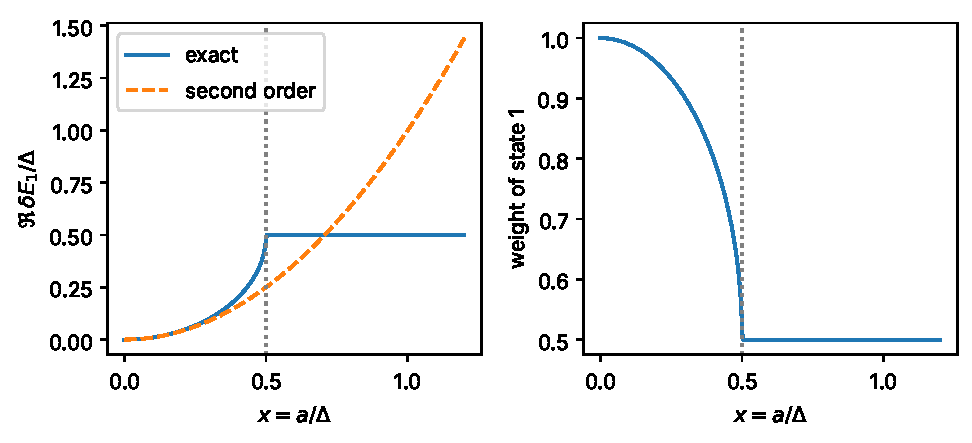
\includegraphics[width=0.95\linewidth]{figs/paper-spurious-floor_twolevel.pdf}
\caption{The two-level model \cref{eq:paper-spurious-floor-2x2}. Left: real shift of the lower level, exact (solid) and second order (dashed), in units of the spacing $\Delta$, against coupling $x=a/\Delta$. The exceptional point at $x=1/2$ is marked; beyond it the exact real shift saturates at $\Delta/2$ while the surrogate keeps growing, overstating the shift twofold at $x=1$. Right: weight of unperturbed state 1 in the lower-branch eigenvector, $|u|^2/(|u|^2+|v'|^2)$; it falls to $1/2$ at the exceptional point and stays there, so the eigenstate can no longer be assigned to a single unperturbed level.}
\label{fig:paper-spurious-floor-twolevel}
\end{figure}

\begin{sample}{Exact versus surrogate in the two-level model}
For \cref{eq:paper-spurious-floor-2x2}, compute the exact and second-order real shifts of the lower level, in units of $\Delta$, at $x=\tfrac14,\tfrac12,1$. Also give $|v'/u|$ for the lower state at $x=\tfrac14$.

\textbf{Step 1: $x=\tfrac14$.} $\sqrt{1-4/16}=\sqrt{0.75}=0.8660$, so $\delta E^{\rm exact}=\tfrac12(1-0.8660)=0.0670$; surrogate $x^2=0.0625$. The surrogate is low by 7\%.

\textbf{Step 2: $x=\tfrac12$.} Exact $\tfrac12(1-0)=0.5$; surrogate $0.25$. At the exceptional point the surrogate understates by a factor two.

\textbf{Step 3: $x=1$.} Exact real part stuck at $0.5$; surrogate $1$. The surrogate now overstates by a factor two.

\textbf{Step 4: overlap.} At $x=\tfrac14$, $|v'/u|=\delta E^{\rm exact}/x=0.0670/0.25=0.268$, so the lower state is clearly state 1.
\[
\boxed{(0.0670,\,0.0625),\ (0.5,\,0.25),\ (0.5,\,1);\quad |v'/u|=0.268}
\]
The model does not prove the paper's "twofold" overstatement; it shows that an overstatement of this size is exactly what happens when a quadratic surrogate is pushed past an exceptional point.
\end{sample}

\begin{sample}{Why quarter amplitude restores agreement}
In the two-level model at $x=0.4$ (below the exceptional point), compute the relative error of the surrogate; repeat at quarter amplitude, $x=0.1$, and compare the ratio of relative errors with the factor 16 suggested by \cref{eq:paper-spurious-floor-series}.

\textbf{Step 1: $x=0.4$.} $\sqrt{1-0.64}=0.6$, exact $=0.2$, surrogate $=0.16$, relative error $(0.16-0.2)/0.2=-0.200$.

\textbf{Step 2: $x=0.1$.} $\sqrt{0.96}=0.97980$, exact $=\tfrac12(0.02020)=0.010102$, surrogate $=0.01$, relative error $-0.0101$.

\textbf{Step 3: ratio.} $0.200/0.0101=19.8$.
\[
\boxed{\text{relative error }-0.200\to-0.0101,\ \text{ratio}\approx19.8}
\]
The ratio is near 16 (the leading $x^2$ scaling), somewhat larger because at $x=0.4$ the higher terms of the series also matter. Quartering the amplitude is a powerful test: if the code were wrong, agreement would not improve like this.
\end{sample}

This is exactly the logic of the paper's next sentence: ``At quarter amplitude the surrogate is accurate (corr $+0.88$/$+0.94$), confirming the machinery and isolating amplitude as the culprit.'' The same tensors, the same code, the same coefficient \emph{direction}: only the size changed. Agreement returned. So the tensors were computed correctly, and the disagreement at full amplitude is due to amplitude alone.

\subsection{The same thing in a many-level box}

\Cref{fig:paper-spurious-floor-boxexact} is a small-scale analogue of the paper's Fig.~5 (left): six random cosine modes in the infinite well, with all 80 basis states, scored on the lowest 40 levels. At small amplitude the exact real shifts (obtained by full complex diagonalization and matched by overlap) lie on the diagonal: their relative rms disagreement with the surrogate is below 5\%. At large amplitude the points leave the diagonal, with relative disagreement above 10\%, because the strongest couplings of the low levels exceed the exceptional-point threshold.

\begin{figure}[htbp]\centering
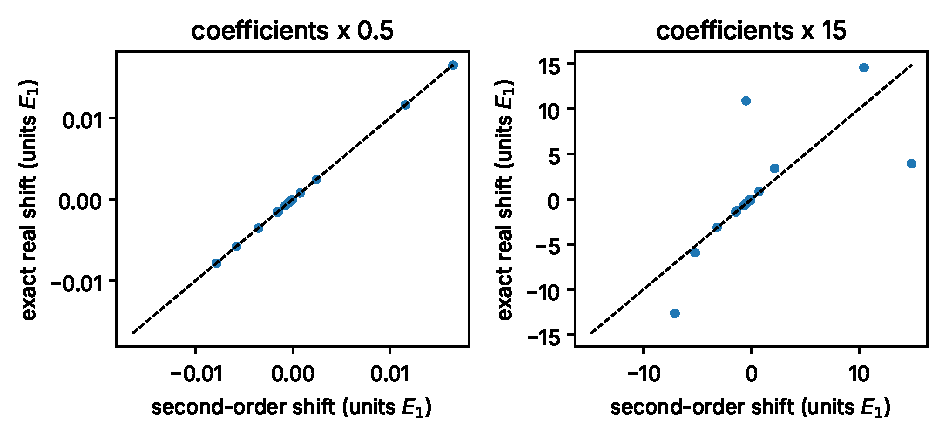
\includegraphics[width=0.95\linewidth]{figs/paper-spurious-floor_boxexact.pdf}
\caption{Exact versus second-order real shifts for $H_0+iA$ in the infinite well ($L=\pi/2$, levels $E_k=k^2$, 80 states), with $A=\sum_{j=1}^{6}c_j\cos(j\pi x/L)$ and random $c_j$ (\texttt{default\_rng(1)}). Exact shifts from dense complex diagonalization, each unperturbed level matched to the eigenvector with largest weight on it; the lowest 40 levels shown. Left: coefficients $0.5c_j$; points on the diagonal. Right: coefficients $15c_j$; the surrogate no longer describes the operator. Energies in units where $E_k=k^2$.}
\label{fig:paper-spurious-floor-boxexact}
\end{figure}

\subsection{Scores worse than the null}

How can a fitted operator score worse than doing nothing? Because its exact shifts are not the surrogate shifts the optimizer tuned. With correlation only $+0.14$ between exact and surrogate, the exact shifts are, for scoring purposes, mostly noise added to the residual.

\begin{sample}{How much noise turns 0.2438 into 0.2523?}
If the exact shifts (in mean spacings) were uncorrelated with the target fluctuations and had rms $\sigma$, what $\sigma$ would turn the null 0.2438 into the paper's exact in-sample scores 0.2523 (odd) and 0.2477 (even)?

\textbf{Step 1: variance addition.} For uncorrelated, mean-zero $d$ and $m$, $\mathrm{rms}(d-m)^2=\mathrm{rms}(d)^2+\sigma^2$.

\textbf{Step 2: solve.} $\sigma=\sqrt{0.2523^2-0.2438^2}=\sqrt{0.063655-0.059438}=\sqrt{0.004217}=0.0649$; and $\sqrt{0.2477^2-0.2438^2}=\sqrt{0.001917}=0.0438$.
\[
\boxed{\sigma\approx0.065\ \text{(odd)},\quad\sigma\approx0.044\ \text{(even)}}
\]
Shifts of only about a twentieth of a spacing, uncorrelated with the target, are enough. (The assumption of zero correlation is an idealization for illustration.)
\end{sample}

\subsection{Wrong-sign widths}

``The fitted absorptive-even solution also violates its physical premise: 58\% of its widths have the wrong sign.'' The even class was meant to model absorption, $\Gamma(x)\ge0$. By \cref{eq:paper-spurious-floor-width}, if $\Gamma\ge0$ everywhere then every first-order width is non-negative; so a negative width proves that $\Gamma(x)<0$ somewhere, i.e.\ the fitted "absorber" amplifies. The paper does not specify whether "widths" means the level widths $\Gamma_n$ or the values of $\Gamma(x)$ on the grid; either reading shows that the unconstrained optimizer ignored the physics the class was designed to represent. That is why the fair version (next section) enforces $\Gamma\ge0$.

\subsection{The cost of exactness}

App.~A step 11: ``dense complex \texttt{eig} of $H+iA$ on $N=2500$, second-order sums over the full grid spectrum, eigenstate matching by overlap with the unperturbed basis.'' A dense eigensolve costs of order $N^3$ operations (Chapter~\ref{ch:eigen}): $2500^3\approx1.6\times10^{10}$, seconds to minutes on a laptop. Note that this check uses a coarser grid than the fits and sums the surrogate over all 2500 grid states, so that exact and surrogate are compared on one common grid, as the paper states in Sec.~II~E (iii).

\begin{checkpoint}
The paper scored the exact spectra in-sample, not out-of-sample. Why is an in-sample score the right test here?
\end{checkpoint}
\checkanswer{The question is whether the floor is a property of an operator at all. The surrogate claimed an in-sample rms of 0.232; if the operator's own spectrum does not reproduce that on the very zeros it was fitted to, the floor belonged to the surrogate. An in-sample failure (0.2523, 0.2477 against 0.2438) settles this without any appeal to generalization.}

\begin{checkpoint}
Why does the PT-odd surrogate's validity break down first at the \emph{lowest} levels in a potential like the box?
\end{checkpoint}
\checkanswer{The validity condition compares couplings with spacings. In the box $E_k=\kappa k^2$, so spacings grow with $k$; the low levels have the smallest spacings and reach the exceptional-point condition (coupling about half the spacing) first. In the Wu--Sprung potential the spacings shrink slowly with height instead, so there the high levels are the more fragile; in either case the condition must be checked level by level.}

\textbf{Strength and limits.} This is the strongest part of the dissection: a direct, exact computation contradicts the surrogate, and a quarter-amplitude control shows the code is right. Limits: the exact check used $N=2500$ rather than the working grid, and, like the rest of Sec.~V, it was not rerun in revision.

\begin{keyideas}
\item The two-level model shows the three symptoms: the surrogate understates at the exceptional point, overstates beyond it (twofold at $a=\Delta$), and eigenvectors become unmatchable.
\item Because real parts are even in amplitude, quartering the amplitude cuts the relative error about sixteenfold; agreement returning at quarter amplitude confirms the code and blames amplitude.
\item Exact in-sample scores 0.2523 and 0.2477 are worse than the null; uncorrelated shifts of rms 0.065 and 0.044 spacings would do this.
\item 58\% wrong-sign widths show the absorptive premise was violated.
\end{keyideas}

%======================================================================
\section{The fair version: amplitude balls and sign constraints}\label{sec:paper-spurious-floor-fair}

\subsection{The claim}

\begin{quote}
``Refitting inside amplitude balls where perturbation theory is verified valid, and with $\Gamma\ge0$ enforced, gives floors within 0.4--4.8\% of the null (Fig.~5, right); the $R=4$ solutions pass exact verification (corr $+0.93$/$+0.995$, all states matched) and their exact-spectrum in-sample gains over the null are 1.9\% (odd) and 0.6\% (even). We conclude that these second-order non-Hermitian families, treated fairly, are empirically inert on this problem.''
\end{quote}

\subsection{The machinery (App.~A step 10, "fair variant")}

\emph{Amplitude ball.} After every LM step, the coefficient vector is projected onto the ball $\norm{c}\le R$:
\begin{equation}
c\;\to\;c\cdot\min\Big(1,\frac{R}{\norm{c}}\Big).\label{eq:paper-spurious-floor-proj}
\end{equation}
This is the closest point of the ball to $c$ (Chapter~\ref{ch:linear-algebra}: for a point outside a sphere, the nearest point of the sphere lies on the line to the center). Restarts are drawn from $\mathcal N(0,(R/20)^2)$, small compared with $R$ so that they start inside the ball. $R$ is "calibrated so that second-order perturbation theory is verified accurate", that is, chosen by checking the surrogate against exact diagonalization.

\emph{Sign penalty} for the absorptive class: the objective gets an extra term $10^4\int\max(A,0)^2\,\dd x$, which is zero when $A\le0$ everywhere (i.e.\ $\Gamma\ge0$) and grows quadratically with any positive excursion.

\begin{sample}{Projection and penalty}
(a) Project $c=(3,4,12)$ onto the ball $\norm c\le4$. (b) For $A(x)=-1+2\cos(\pi x/L)$ on $[-L,L]$ with $L=44.883$ (RE3), compute the penalty $10^4\int\max(A,0)^2\,\dd x$.

\textbf{Step 1: norm.} $\norm c=\sqrt{9+16+144}=13$.

\textbf{Step 2: scale.} $c\to(4/13)(3,4,12)=(0.923,\,1.231,\,3.692)$.

\textbf{Step 3: where $A>0$.} $\cos(\pi x/L)>\tfrac12$ means $|\pi x/L|<\pi/3$. Substitute $\theta=\pi x/L$, $\dd x=(L/\pi)\dd\theta$.

\textbf{Step 4: integrate.} $(2\cos\theta-1)^2=4\cos^2\theta-4\cos\theta+1=3+2\cos2\theta-4\cos\theta$, so
\[
\int_{-\pi/3}^{\pi/3}(2\cos\theta-1)^2\dd\theta=\Big[3\theta+\sin2\theta-4\sin\theta\Big]_{-\pi/3}^{\pi/3}
=2\Big(\pi+\frac{\sqrt3}{2}-2\sqrt3\Big)=2\pi-3\sqrt3=1.0870 .
\]
\textbf{Step 5: penalty.} $\int\max(A,0)^2\dd x=(L/\pi)(2\pi-3\sqrt3)=14.287\times1.0870=15.53$, so the penalty is $1.553\times10^5$.
\[
\boxed{c\to(0.923,1.231,3.692);\qquad\text{penalty}\approx1.55\times10^5}
\]
A penalty this large dwarfs an rms objective of order $0.06$ (squared), so the optimizer is pushed hard toward $A\le0$.
\end{sample}

\subsection{The results}

From the key anchors of App.~A: fair $R=4$ surrogate floors $0.2335$ (odd) and $0.2422$ (even); exact-verified in-sample scores $0.2391$ and $0.2423$. As percentages of the null 0.2438 (Problem~13), the surrogate floors capture 4.2\% and 0.66\% and the exact spectra 1.9\% and 0.6\%. These sit inside the paper's quoted range "within 0.4--4.8\% of the null" for the surrogate floors over the ball sizes tried. And at $R=4$ the surrogate is trustworthy: correlation with exact shifts $+0.93$ and $+0.995$, every eigenstate matched.

\textbf{In plain words.} When the model is kept in the regime where its own formula is correct, and when the absorber is forced to absorb, it improves on doing nothing by about one or two percent. That is what "empirically inert" means.

\textbf{Strength and limits.} The fair refit is the right control: it gives the model class every chance consistent with its own validity. But it tests two classes, one background, one optimizer and one set of ball sizes; the word "inert" is the paper's summary for these, "on this problem," and should not be stretched to non-Hermitian operators in general. The paper itself scopes it: ``these second-order non-Hermitian families, treated fairly.''

\begin{checkpoint}
Why restart from $\mathcal N(0,(R/20)^2)$ rather than from $\mathcal N(0,0.3^2)$ as in the unconstrained fits?
\end{checkpoint}
\checkanswer{To start inside the region where the surrogate is valid. A start far outside the ball would immediately be projected onto its surface, and the restarts would no longer sample the interior; scaling the spread with $R$ keeps the restarts meaningful for every ball size.}

\begin{keyideas}
\item The fair version projects $c$ onto $\norm c\le R$ after every step, penalizes $A>0$ with weight $10^4$, and restarts inside the ball.
\item At $R=4$ the surrogate is verified (corr $+0.93$/$+0.995$, all states matched); exact in-sample gains are 1.9\% (odd) and 0.6\% (even).
\item Conclusion, scoped: these families, treated fairly, are empirically inert on this problem.
\end{keyideas}

%======================================================================
\section{General lessons for computational science}\label{sec:paper-spurious-floor-lessons}

The paper closes Sec.~V with a general statement:

\begin{quote}
``Each ingredient of the spurious floor is generic in computational and machine-learned science: surrogate optimization outside its validity region, dead parameters coupling to numerical noise, and shared constants across model variants mistaken for physics. A surrogate improvement is not an operator-level result until the exact spectrum of the fitted operator confirms it.''
\end{quote}

Each ingredient has a cheap detector, and you have now seen all of them work.

\begin{enumerate}
\item \textbf{Surrogate outside its validity region.} Detector: score the exact model at the fitted parameters, and repeat at reduced amplitude. If agreement returns at reduced amplitude, the code is right and the amplitude is wrong. (\Cref{sec:paper-spurious-floor-exact}.)
\item \textbf{Dead parameters coupling to noise.} Detector: list every parameter that should have no effect, check analytically that its derivatives vanish, set them to exact zeros, and look at fitted coefficient magnitudes; a coefficient of $2.2\times10^6$ is a symptom, not a result. Recompute in higher precision. (\Cref{sec:paper-spurious-floor-nullmode}.)
\item \textbf{Shared constants mistaken for physics.} Detector: when two variants agree suspiciously well, ask what they share (code, optimizer, data type, defaults) and break the shared part. (\Cref{sec:paper-spurious-floor-nullmode}.)
\item \textbf{A plausible mechanism.} Detector: make the mechanism quantitative before believing it. The block-coherence idea was natural and wrong by a factor of 2 to 7. (\Cref{sec:paper-spurious-floor-blocks}.)
\item \textbf{Physical constraints.} Detector: check that fitted parameters respect the premise of the model (58\% wrong-sign widths). (\Cref{sec:paper-spurious-floor-exact}.)
\end{enumerate}

Item 1 reappears as point (ii) of the paper's falsifiability standard in Sec.~VI: ``scoring of the actual operator spectrum, not a surrogate.'' Section~V is the paper's own evidence for why that point belongs on the list.

\begin{pitfall}
"Exact" here means exact for the discretized operator: dense diagonalization of the finite-difference matrix. It does not remove discretization error. That is a separate issue, handled in the Hermitian part of the paper by bias-corrected targets (Chapter~\ref{ch:finite-differences}).
\end{pitfall}

\begin{keyideas}
\item The three generic ingredients: surrogate outside validity, dead parameters on noise, shared constants read as physics.
\item Each has a cheap detector: exact scoring plus reduced amplitude; analytic zeros and coefficient inspection; breaking shared components.
\item Section~V motivates point (ii) of the paper's proposed standard.
\end{keyideas}

%======================================================================
\section{Paper connection}\label{sec:paper-spurious-floor-paper}

This section lists, in paper order, every place the material of this chapter appears in R1 \cite{soniR1}.

\textbf{Abstract.} One sentence: ``A subsidiary dissection of second-order non-Hermitian perturbations shows how surrogate optimization outside its validity range can manufacture an apparently meaningful in-sample floor; exact diagonalization dissolves it.'' Every word is now unpacked: "subsidiary" (\cref{sec:paper-spurious-floor-scope}), "surrogate" (\cref{sec:paper-spurious-floor-surrogate}), "outside its validity range" (\cref{sec:paper-spurious-floor-exact}), "apparently meaningful floor" (\cref{sec:paper-spurious-floor-floors,sec:paper-spurious-floor-nullmode}).

\textbf{Sec.~II~E, "Second-order non-Hermitian classes, amplitude control, and exact diagonalization."} Defines $H\to H+iA$, the PT-odd class $\phi_k=\sin((k+1)\pi x/L)$ with $A_{nn}=0$, and the absorptive-even class $\phi_k=\cos(k\pi x/L)$ modeling $-i\Gamma/2$ (our \cref{eq:paper-spurious-floor-odd,eq:paper-spurious-floor-even,eq:paper-spurious-floor-GammaA}). Eq.~(5) is our \cref{eq:paper-spurious-floor-eq5,eq:paper-spurious-floor-T}; the state sum over 652 states and the 500-state bias are \cref{fig:paper-spurious-floor-truncation}. Safeguards (i) null mode (\cref{sec:paper-spurious-floor-nullmode}), (ii) amplitude balls and $\Gamma\ge0$ (\cref{sec:paper-spurious-floor-fair}), (iii) exact diagonalization with overlap matching (\cref{sec:paper-spurious-floor-exact}). Notation overloads: $A$ (operator) versus $A_{nk}$ of Sec.~II~C; $T^{(n)}$ versus the window $T$ of Sec.~II~D and $T_k$ of the Chebyshev basis.

\textbf{Sec.~V, first paragraph.} Floors 0.2321, 0.2358 (repaired), 0.2322 (artifact), null 0.2438, OOS rms up to 1.4 and 167, $c_0\approx2.2\times10^6$: \cref{sec:paper-spurious-floor-floors,sec:paper-spurious-floor-nullmode}, \cref{fig:paper-spurious-floor-floors}.

\textbf{Sec.~V, "The proposed mechanism fails quantitatively."} Sum rule to $4\times10^{-15}$, locality, block-coherent rms 0.03--0.11 for windows 3--13, factor 2--7, $p=2$ period $\approx9$ in $t$ and 6--7 levels, capture 3--7\%: \cref{sec:paper-spurious-floor-blocks}, \cref{fig:paper-spurious-floor-blocks}.

\textbf{Sec.~V, "The optimizer left the perturbative regime."} Correlations $+0.14$/$+0.18$, twofold overstatement, 3\% unmatched, exact scores 0.2523/0.2477, quarter-amplitude correlations $+0.88$/$+0.94$, 58\% wrong-sign widths: \cref{sec:paper-spurious-floor-exact}, \cref{fig:paper-spurious-floor-twolevel,fig:paper-spurious-floor-boxexact}.

\textbf{Sec.~V, "The fair version captures almost nothing."} Floors within 0.4--4.8\% of the null, $R=4$ correlations $+0.93$/$+0.995$, exact gains 1.9\%/0.6\%: \cref{sec:paper-spurious-floor-fair}.

\textbf{Sec.~V, closing paragraph.} The three generic ingredients: \cref{sec:paper-spurious-floor-lessons}.

\textbf{Sec.~V~A, "Sum rule and locality details."} Sum-rule values $3.6\times10^{-15}$ and $1.4\times10^{-14}$; weights $w_{nm}=|A_{nm}|^2/|E_n-E_m|$ with half within $|n-m|\le5$ (odd) and $\le10$ (even), 90\% within about 60 levels; block-coherent rms 0.108, 0.049, 0.033, 0.035, 0.019 for $w=3,5,7,9,13$; output correlation $\approx+0.3$ with rms 0.06--0.075: \cref{sec:paper-spurious-floor-blocks}.

\textbf{Fig.~5.} Left panel (exact versus second-order shifts, unconstrained PT-odd fit) is reproduced in spirit by our \cref{fig:paper-spurious-floor-boxexact}; right panel (in-sample floors under amplitude control, "$R=4$ exact") corresponds to the right half of our \cref{fig:paper-spurious-floor-floors}.

\textbf{Appendix~A, step 9.} Tensors with $\psi$ normalized by $\sum\psi^2\dd x=1$; $T^{(n)}$ over 652 states; even-class rows $T^{(n)}_{0l}$ zeroed analytically. \textbf{Step 10.} LM on $r_n=(\mathrm{fluc}_n+c^\top T^{(n)}c)/\gap_n$, Jacobian $2(T^{(n)}c)_k/\gap_n$, try-list $(0.3\lambda,\lambda,10\lambda)$ with diag scaling, 6 restarts $c\sim\mathcal N(0,0.3^2)^M$, seed 0, at most 200 iterations; fair variant with projection onto $\norm c\le R$, restarts $\mathcal N(0,(R/20)^2)$, sign penalty $10^4\int\max(A,0)^2\dd x$. \textbf{Step 11.} Dense complex \texttt{eig} on $N=2500$, matching by overlap. \textbf{Step 4} supplies the 652 states (eigenvalue range $[0,1000]$ for tensors).

\textbf{Key anchors.} Unconstrained floors $0.2321$/$0.2358$ ($0.2322$ with artifact); exact-spectrum in-sample $0.2523$/$0.2477$; fair $R=4$ floors $0.2335$/$0.2422$; exact-verified $0.2391$/$0.2423$; in-sample null $0.2438$.

\textbf{Sec.~VI.} ``The non-Hermitian analysis of Sec.~V is inherited from the original computation and was not rerun for this revision.'' Also point (ii) of the proposed standard. Chapter~\ref{ch:paper-critique} weighs these.

\textbf{Sec.~II~F.} The pipeline, including this part, was written and analyzed with substantial assistance from a large language model, under the author's direction and review; reproducibility from the archived record \cite{zenodo} is what makes the numbers above checkable.

%======================================================================
\section{Summary}

\begin{itemize}
\item Section~V is a subsidiary method stress test; the Hermitian conclusions do not depend on it; it was not rerun in revision.
\item The surrogate Eq.~(5), $\delta E_n=-\sum_{m\ne n}A_{nm}^2/(E_n-E_m)=-c^\top T^{(n)}c$, follows from second-order perturbation theory with $W=iA$ (\cref{eq:paper-spurious-floor-RS2,eq:paper-spurious-floor-eq5,eq:paper-spurious-floor-T}); coupled levels attract.
\item Real parts of eigenvalues are even in the amplitude (\cref{eq:paper-spurious-floor-even-odd}); the surrogate's relative error grows as amplitude squared; PT-odd spectra stay exactly real until a collision.
\item One cosine in the box gives $\delta E_n=-c^2/(8\kappa(n^2-j^2))$ (\cref{eq:paper-spurious-floor-onemode}); truncating the state sum biases the top levels.
\item Unconstrained floors 0.2321 (odd) and 0.2358 (even) against null 0.2438 are captures of 4.8\% and 3.3\%; OOS predictions are useless and can explode.
\item The constant mode is exactly null (\cref{eq:paper-spurious-floor-constshift,eq:paper-spurious-floor-T0l}); in float32 it coupled to noise with $c_0\approx2.2\times10^6$ and produced the spurious 0.2322; least squares harvests a fixed gain from any noise column.
\item The sum rule (\cref{eq:paper-spurious-floor-sumrule}) and locality make the block-coherent rms a lower bound on a local model's residual; it is far below the floor, so the block-coherence mechanism fails; the floor is a small capture.
\item The two-level model (\cref{eq:paper-spurious-floor-2x2eig,eq:paper-spurious-floor-2x2shift}) shows the exceptional point, twofold overstatement past it, and loss of overlap matching.
\item Exact spectra of the unconstrained fits score 0.2523/0.2477, worse than the null; at quarter amplitude the surrogate is accurate.
\item The fair refit (\cref{eq:paper-spurious-floor-proj}, sign penalty) gains 1.9\%/0.6\% in exact spectra: these families are empirically inert on this problem.
\item Generic lesson: a surrogate improvement is not an operator-level result until the exact spectrum confirms it.
\end{itemize}

%======================================================================
\section{Problems}

\begin{problemlist}
\prob{1}{Using the paper's numbers (Sec.~V), compute by what percentage the exact-spectrum in-sample scores of the unconstrained fits, 0.2523 (odd) and 0.2477 (even), exceed the null 0.2438.}

\prob{1}{In two or three sentences, explain why the paper calls Eq.~(5) a "surrogate" and an "optimization device", and what object a physical claim must be about.}

\prob{1}{Starting from $V(x)-i\Gamma(x)/2=V(x)+iA(x)$, show that the physical requirement $\Gamma\ge0$ is equivalent to $A\le0$ pointwise.}

\prob{2}{In the box with $L=\pi/2$ ($E_k=k^2$), take a single cosine mode with $j=2$ and $c=1$. Using \cref{eq:paper-spurious-floor-boxcos}, list the coupling partners of levels $n=1,\dots,6$ and compute $\delta E_n$ for each, treating $n=j=2$ and $n=2j=4$ separately.}

\prob{2}{Show that $T^{(n)}_{kl}$ in \cref{eq:paper-spurious-floor-T} is symmetric in $k$ and $l$, and derive $\partial(c^\top Tc)/\partial c_k=2(Tc)_k$. Then evaluate $r_n$ and the Jacobian row for $T^{(n)}=\begin{pmatrix}1&0.5\\0.5&2\end{pmatrix}$, $c=(2,1)$, $\mathrm{fluc}_n=0.3$, $\gap_n=1.2$.}

\prob{2}{Suppose the computed overlaps $(\phi_0)_{nm}$ carry noise of typical size $\eta$. Estimate the size of $c_0$ needed for the effective matrix $c_0\eta_{nm}$ to reach $0.1$ in energy units, for $\eta=10^{-8}$ and for $\eta=10^{-16}$. What does the second answer tell you about float64?}

\prob{2}{Using qmnt, compute $\gap_n$ at $n=100$, $300$ and $400$ and the number of levels spanned by one period $2\pi/\log2$ of the $p=2$ oscillation at each height. Is the paper's "6--7 levels at these heights" consistent with your numbers for zeros 1--400?}

\prob{2}{For the two-level model \cref{eq:paper-spurious-floor-2x2} at $x=a/\Delta=0.3$, compute the exact and second-order real shifts of the lower level in units of $\Delta$, and the relative error of the surrogate.}

\prob{2}{Three levels $E=(0,1,3)$ are coupled by a real symmetric $A$ with $A_{12}=0.1$, $A_{23}=0.2$, $A_{13}=0.05$ and zero diagonal. Compute the three second-order real shifts under $H\to H+iA$ and verify the sum rule.}

\prob{2}{For $d_n=(-1)^na$ with $a=0.24$, compute the block-coherent rms for $w=3$ and $w=5$ using the result of the sample problem on negatively correlated sequences. Compare with the paper's $w=3$ value 0.108 and comment.}

\prob{2}{Using qmnt, compute $d_n=(t_n-s_n)/\gap_n$ for $n=1,\dots,400$ and the rms of its centred $w$-level moving average (full windows only) for $w=3,5,7,9,13$. Compare with the paper's Sec.~V~A values and with the floor 0.232.}

\prob{2}{Using numpy, repeat the "harvesting a noise column" sample with $\varepsilon=10^{-3}$ and $\varepsilon=10^{-9}$. Report the coefficient $\beta_z$ and the rms residual in each case, and explain why the rms does not change.}

\prob{1}{Using the key anchors of App.~A, express the fair $R=4$ surrogate floors (0.2335 odd, 0.2422 even) and the exact-verified scores (0.2391, 0.2423) as percentage improvements over the null 0.2438.}

\prob{2}{For a general $2\times2$ matrix $\begin{pmatrix}E_1&ia\\ia&E_2\end{pmatrix}$ with $E_2>E_1$ and real $a$, find the value of $a$ at which the exceptional point occurs, and the common eigenvalue there.}

\prob{3}{Expand the exact two-level shift \cref{eq:paper-spurious-floor-2x2shift} to sixth order in $x$. Confirm that no odd powers appear and give the coefficients of $x^4$ and $x^6$.}

\prob{2}{Using numpy, build $H_0+iA$ for the box ($E_k=k^2$, 80 states) with $A=c\cos(\pi x/L)$, and compare exact and second-order real shifts of the lowest 10 levels at $c=8$ and at $c=2$ (quarter amplitude). By roughly what factor does the relative error drop?}

\prob{3}{Generalize the argument of \cref{eq:paper-spurious-floor-conj,eq:paper-spurious-floor-even-odd}: show that for any real symmetric $H_0$ and real symmetric $A$, the characteristic polynomial $\det(H_0+iaA-\lambda)$ has real coefficients when $a$ is replaced by $ia'$ with $a'$ real, and use this to explain once more why only even powers of $a$ appear in the real parts.}

\prob{2}{Redo the weak-capture sample problem with correlation $\rho=0.2$ instead of $0.3$. What is the optimal output rms and the resulting residual rms? Does this still land near the paper's floors?}

\prob{2}{From the paper's Sec.~V~A block-coherent values (0.108, 0.049, 0.033, 0.035, 0.019 for $w=3,5,7,9,13$), compute the ratio $0.232/\mathrm{rms}(B_w)$ for each window. Which windows give the paper's quoted range "2--7"?}

\prob{3}{Design, in words, a test that would have caught the null-mode artifact even if nobody had noticed $c_0\approx2.2\times10^6$. Your test must use only the fitted model and the data, and should be cheap.}

\prob{3}{The paper reports that 3\% of eigenstates could not be matched one-to-one at the fitted amplitude. Using the two-level model, explain why an unmatched state signals that at least one pair of levels has passed (or is near) an exceptional point, and why such levels make the surrogate shifts meaningless for that pair.}
\end{problemlist}

%======================================================================
\section{Answers to selected problems}

\textbf{1.} $0.2523/0.2438=1.0349$, so 3.49\% worse; $0.2477/0.2438=1.0160$, so 1.60\% worse. Both exact spectra are worse than doing nothing.

\textbf{2.} Eq.~(5) is a cheap approximate formula for the real level shifts, used in place of the exact eigenvalues during optimization. It is only valid while couplings are small compared with spacings. A physical claim must be about the exact spectrum of the fitted operator $H+iA$.

\textbf{3.} Equate imaginary parts: $-\Gamma/2=A$, so $A=-\Gamma/2$. Since $-\tfrac12<0$, $\Gamma(x)\ge0$ holds at a point exactly when $A(x)\le0$ there.

\textbf{5.} $T_{kl}$ contains the product $(\phi_k)_{nm}(\phi_l)_{nm}$, symmetric under $k\leftrightarrow l$. The derivative is \cref{eq:paper-spurious-floor-grad}. Numbers: $Tc=(2.5,3)$, $c^\top Tc=8$, $r_n=(0.3+8)/1.2=6.917$, $J=2(2.5,3)/1.2=(4.167,5.000)$.

\textbf{7.} $\sqrt{1-0.36}=0.8$, exact $=0.1\Delta$; surrogate $=0.09\Delta$; relative error $-10\%$.

\textbf{9.} $w=3$: $q=1$, rms $a/3=0.080$; $w=5$: $a/5=0.048$. The paper's 0.108 at $w=3$ is somewhat larger than for a perfectly alternating sequence of the same amplitude: the zeros are negatively correlated but not perfectly alternating, so some slow component survives. Both are far below 0.232.

\textbf{11.} Every value stays below 0.15 (the CHECKS script asserts this for $w\ge3$), decreasing broadly with $w$, comparable to the paper's values and several times below 0.232. Small differences come from using $s_n$ rather than the paper's Richardson-corrected targets.

\textbf{13.} Surrogate: $(0.2438-0.2335)/0.2438=4.22\%$, $(0.2438-0.2422)/0.2438=0.66\%$. Exact: $1.93\%$ and $0.62\%$, matching the paper's 1.9\% and 0.6\%.

\textbf{15.} With $u=4x^2$, $\sqrt{1-u}=1-\tfrac u2-\tfrac{u^2}8-\tfrac{u^3}{16}-\dots=1-2x^2-2x^4-4x^6-\dots$, so $\delta E_1^{\rm exact}=\tfrac\Delta2(2x^2+2x^4+4x^6)=\Delta(x^2+x^4+2x^6)+\dots$. Only even powers; coefficients 1 and 2.

\textbf{17.} Sketch: in the real basis, $(H_0+iaA)^*=H_0-iaA$, so the polynomial $p_a(\lambda)=\det(H_0+iaA-\lambda)$ satisfies $\overline{p_a(\bar\lambda)}=p_{-a}(\lambda)$. Setting $a=ia'$ makes the matrix $H_0-a'A$ real, so its coefficients are real. The roots continuing $E_n$ are therefore real-analytic in $a'$; in terms of $a$, $a'=-ia$, so terms odd in $a$ carry a factor $i$ and contribute only to imaginary parts, even terms only to real parts. Same conclusion as \cref{eq:paper-spurious-floor-series}.

\textbf{19.} $0.232/0.108=2.15$, $/0.049=4.73$, $/0.033=7.03$, $/0.035=6.63$, $/0.019=12.2$. Windows 3--9 give 2.1--7.0, the quoted "2--7"; $w=13$ gives about 12, outside the quoted range but strengthening the conclusion.
